% Options for packages loaded elsewhere
\PassOptionsToPackage{unicode}{hyperref}
\PassOptionsToPackage{hyphens}{url}
%
\documentclass[
]{book}
\usepackage{amsmath,amssymb}
\usepackage{lmodern}
\usepackage{iftex}
\ifPDFTeX
  \usepackage[T1]{fontenc}
  \usepackage[utf8]{inputenc}
  \usepackage{textcomp} % provide euro and other symbols
\else % if luatex or xetex
  \usepackage{unicode-math}
  \defaultfontfeatures{Scale=MatchLowercase}
  \defaultfontfeatures[\rmfamily]{Ligatures=TeX,Scale=1}
\fi
% Use upquote if available, for straight quotes in verbatim environments
\IfFileExists{upquote.sty}{\usepackage{upquote}}{}
\IfFileExists{microtype.sty}{% use microtype if available
  \usepackage[]{microtype}
  \UseMicrotypeSet[protrusion]{basicmath} % disable protrusion for tt fonts
}{}
\makeatletter
\@ifundefined{KOMAClassName}{% if non-KOMA class
  \IfFileExists{parskip.sty}{%
    \usepackage{parskip}
  }{% else
    \setlength{\parindent}{0pt}
    \setlength{\parskip}{6pt plus 2pt minus 1pt}}
}{% if KOMA class
  \KOMAoptions{parskip=half}}
\makeatother
\usepackage{xcolor}
\IfFileExists{xurl.sty}{\usepackage{xurl}}{} % add URL line breaks if available
\IfFileExists{bookmark.sty}{\usepackage{bookmark}}{\usepackage{hyperref}}
\hypersetup{
  pdftitle={Etude Finale SPR},
  pdfauthor={Innovations \& Entreprenariat Social},
  hidelinks,
  pdfcreator={LaTeX via pandoc}}
\urlstyle{same} % disable monospaced font for URLs
\usepackage{longtable,booktabs,array}
\usepackage{calc} % for calculating minipage widths
% Correct order of tables after \paragraph or \subparagraph
\usepackage{etoolbox}
\makeatletter
\patchcmd\longtable{\par}{\if@noskipsec\mbox{}\fi\par}{}{}
\makeatother
% Allow footnotes in longtable head/foot
\IfFileExists{footnotehyper.sty}{\usepackage{footnotehyper}}{\usepackage{footnote}}
\makesavenoteenv{longtable}
\usepackage{graphicx}
\makeatletter
\def\maxwidth{\ifdim\Gin@nat@width>\linewidth\linewidth\else\Gin@nat@width\fi}
\def\maxheight{\ifdim\Gin@nat@height>\textheight\textheight\else\Gin@nat@height\fi}
\makeatother
% Scale images if necessary, so that they will not overflow the page
% margins by default, and it is still possible to overwrite the defaults
% using explicit options in \includegraphics[width, height, ...]{}
\setkeys{Gin}{width=\maxwidth,height=\maxheight,keepaspectratio}
% Set default figure placement to htbp
\makeatletter
\def\fps@figure{htbp}
\makeatother
\setlength{\emergencystretch}{3em} % prevent overfull lines
\providecommand{\tightlist}{%
  \setlength{\itemsep}{0pt}\setlength{\parskip}{0pt}}
\setcounter{secnumdepth}{5}
\usepackage{booktabs}
\usepackage{booktabs}
\usepackage{longtable}
\usepackage{array}
\usepackage{multirow}
\usepackage{wrapfig}
\usepackage{float}
\usepackage{colortbl}
\usepackage{pdflscape}
\usepackage{tabu}
\usepackage{threeparttable}
\usepackage{threeparttablex}
\usepackage[normalem]{ulem}
\usepackage{makecell}
\usepackage{xcolor}
\ifLuaTeX
  \usepackage{selnolig}  % disable illegal ligatures
\fi
\usepackage[]{natbib}
\bibliographystyle{apalike}

\title{Etude Finale SPR}
\author{Innovations \& Entreprenariat Social}
\date{2021-07-06}

\begin{document}
\maketitle

{
\setcounter{tocdepth}{1}
\tableofcontents
}
\hypertarget{introduction}{%
\chapter{Introduction}\label{introduction}}

Ce site nous permettra de suivre en temps réel la situation de récolte et d'analyse des données en cours de reolcte

Il constitue un moyen de vérification à temps réel de l'évalution de collecte, de l'assurance qualité des donnnes et de la performance des activités sur terrain.

\hypertarget{data-monitoring}{%
\chapter{Data Monitoring}\label{data-monitoring}}

\hypertarget{carte-de-lenquete}{%
\section{Carte de l'enquete}\label{carte-de-lenquete}}

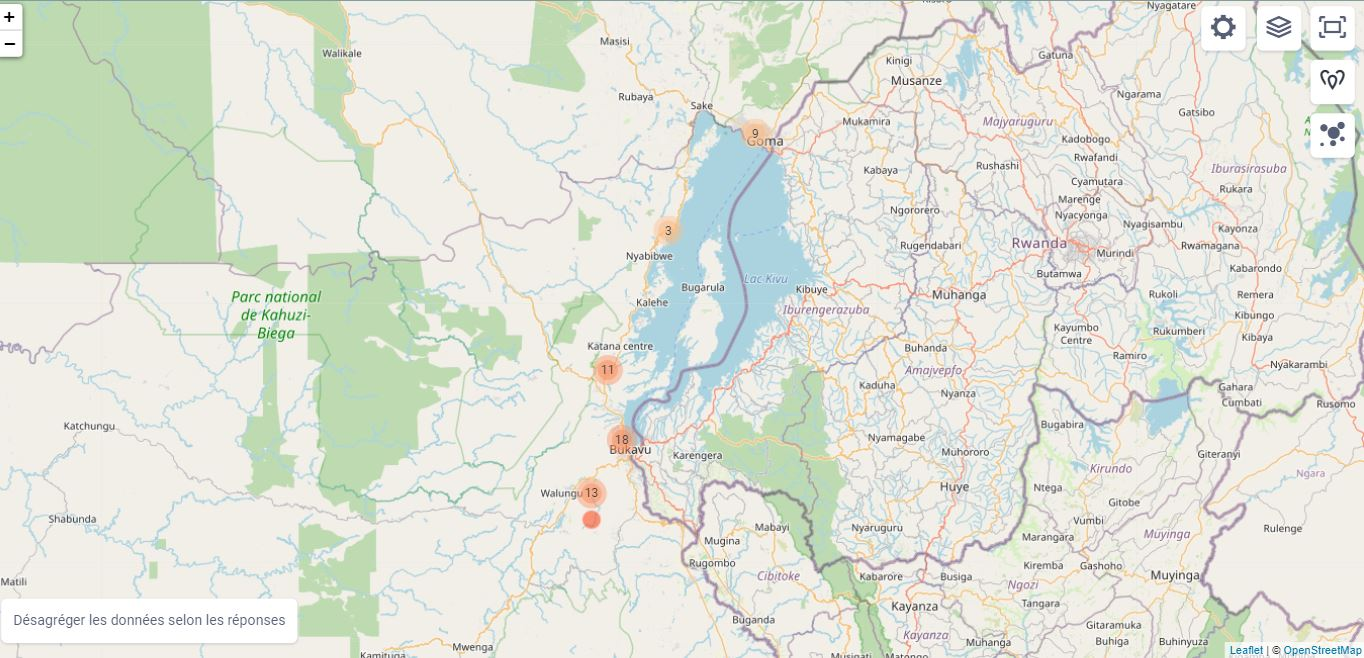
\includegraphics{Carte_enquete.JPG}
Image construite suite aux points géographiques recoltées dans l'Etude Finale sur la Cohésion Sociale du Projet SPR

\hypertarget{analyse-des-donnes}{%
\section{Analyse des donnes}\label{analyse-des-donnes}}

création de la variable durée

Analyse des durée d'enquete pour le premier Jour

Temps moyen par enqueteur

\begin{verbatim}
## `summarise()` has grouped output by 'nom_enqueteur', 'Village'. You can override using the `.groups` argument.
\end{verbatim}

\begin{tabu} to \linewidth {>{\raggedright}X>{\raggedright}X>{\raggedright}X>{\raggedleft}X}
\hline
nom\_enqueteur & Village & date\_enq & temps\_moyen\\
\hline
agnes & n/a & 2021-07-05 & 64.16667\\
\hline
agnes & n/a & 2021-07-06 & 49.90000\\
\hline
aziza & n/a & 2021-07-05 & 38.66667\\
\hline
aziza & n/a & 2021-07-06 & 31.41667\\
\hline
brigitte & KABULU I & 2021-07-05 & 33.42857\\
\hline
brigitte & KABULU I & 2021-07-06 & 151.00000\\
\hline
brigitte & NYABIBWE CENTRE & 2021-07-04 & 142.40000\\
\hline
brigitte & NYABIBWE CENTRE & 2021-07-06 & 173.80000\\
\hline
cidorho cirhulwire & CIHERANO & 2021-07-04 & 98.87500\\
\hline
cidorho cirhulwire & KAHANDA & 2021-07-06 & 43.55556\\
\hline
cidorho cirhulwire & LURHALA CENTRE & 2021-07-05 & 46.25000\\
\hline
cikuru emmanuel & n/a & 2021-07-04 & 349.12500\\
\hline
cikuru emmanuel & n/a & 2021-07-05 & 61.18182\\
\hline
eloi zihalirwa eloi & BULOHO II & 2021-07-05 & 39.00000\\
\hline
elvis & KABULU I & 2021-07-05 & 368.00000\\
\hline
gratiane hamuli & KABULU I & 2021-07-05 & 218.28571\\
\hline
gratiane hamuli & KABULU I & 2021-07-06 & 199.80000\\
\hline
gratiane hamuli & NYABIBWE CENTRE & 2021-07-04 & 160.75000\\
\hline
gratiane hamuli & NYABIBWE CENTRE & 2021-07-06 & 199.50000\\
\hline
haleine & n/a & 2021-07-05 & 55.60000\\
\hline
haleine & n/a & 2021-07-06 & 37.41667\\
\hline
iragi & BULOHO I & 2021-07-05 & 34.66667\\
\hline
iragi & BULOHO II & 2021-07-05 & 50.66667\\
\hline
iragi & BWIMIKA & 2021-07-06 & 42.88889\\
\hline
iragi & KABALE & 2021-07-05 & 96.00000\\
\hline
iragi & KARHANDA & 2021-07-04 & 46.50000\\
\hline
iragi olivier & BULOHO I & 2021-07-05 & 51.25000\\
\hline
iragi olivier & BULOHO II & 2021-07-05 & 40.20000\\
\hline
iragi olivier & BWIMIKA & 2021-07-06 & 39.42857\\
\hline
iragi olivier & KARHANDA & 2021-07-04 & 238.00000\\
\hline
iragi olivier & KARHANDA & 2021-07-06 & 38.00000\\
\hline
irene & CIHERANO & 2021-07-04 & 111.66667\\
\hline
irene & KAHANDA & 2021-07-06 & 46.83333\\
\hline
irene & LURHALA CENTRE & 2021-07-05 & 82.25000\\
\hline
muhindo & KALINGA & 2021-07-06 & 43.71429\\
\hline
ohirwe oluhya & n/a & 2021-07-04 & 283.37500\\
\hline
ohirwe oluhya & n/a & 2021-07-05 & 45.11111\\
\hline
ohirwe oluhya & n/a & 2021-07-06 & 46.55556\\
\hline
pascal & KALINGA & 2021-07-06 & 59.71429\\
\hline
prudent murhula & KABULU I & 2021-07-05 & 54.20000\\
\hline
prudent murhula & KABULU I & 2021-07-06 & 37.60000\\
\hline
prudent murhula & NYABIBWE CENTRE & 2021-07-04 & 90.84615\\
\hline
prudent murhula & NYABIBWE CENTRE & 2021-07-05 & 44.50000\\
\hline
prudent murhula & NYABIBWE CENTRE & 2021-07-06 & 37.50000\\
\hline
riziki mongane solange & CIHERANO & 2021-07-04 & 42.85714\\
\hline
riziki mongane solange & KAHANDA & 2021-07-06 & 48.37500\\
\hline
riziki mongane solange & LURHALA CENTRE & 2021-07-05 & 43.22222\\
\hline
rosette & KALINGA & 2021-07-06 & 63.83333\\
\hline
rosine & BULOHO I & 2021-07-05 & 43.60000\\
\hline
rosine & BULOHO II & 2021-07-05 & 40.50000\\
\hline
rosine & BWIMIKA & 2021-07-06 & 39.77778\\
\hline
rosine & KARHANDA & 2021-07-04 & 188.16667\\
\hline
rosine & KARHANDA & 2021-07-06 & 40.00000\\
\hline
solange riziki mongane solange & CIHERANO & 2021-07-04 & 56.00000\\
\hline
\end{tabu}

\hypertarget{ruxe9sumuxe9-des-donnuxe9es-ruxe9coltuxe9es-duxe9sagruxe9guxe9es-selon-le-sexe-des-enquetuxe9s}{%
\section{Résumé des données récoltées désagrégées selon le sexe des enquetés}\label{ruxe9sumuxe9-des-donnuxe9es-ruxe9coltuxe9es-duxe9sagruxe9guxe9es-selon-le-sexe-des-enquetuxe9s}}

\begin{tabular}{l|l|l}
\hline
**Caractéristique** & **Femme**, N = 180 & **Homme**, N = 158\\
\hline
temps & 43 (36 – 61) & 46 (35 – 66)\\
\hline
nom\_enqueteur &  & \\
\hline
prudent murhula & 13 (7·2\%) & 18 (11\%)\\
\hline
ohirwe oluhya & 14 (7·8\%) & 12 (7·6\%)\\
\hline
cidorho cirhulwire & 14 (7·8\%) & 11 (7·0\%)\\
\hline
rosine & 15 (8·3\%) & 10 (6·3\%)\\
\hline
iragi & 13 (7·2\%) & 11 (7·0\%)\\
\hline
iragi olivier & 13 (7·2\%) & 11 (7·0\%)\\
\hline
riziki mongane solange & 14 (7·8\%) & 10 (6·3\%)\\
\hline
irene & 12 (6·7\%) & 11 (7·0\%)\\
\hline
gratiane hamuli & 3 (1·7\%) & 19 (12\%)\\
\hline
brigitte & 19 (11\%) & 2 (1·3\%)\\
\hline
cikuru emmanuel & 11 (6·1\%) & 8 (5·1\%)\\
\hline
aziza & 10 (5·6\%) & 8 (5·1\%)\\
\hline
haleine & 11 (6·1\%) & 6 (3·8\%)\\
\hline
agnes & 7 (3·9\%) & 9 (5·7\%)\\
\hline
muhindo & 3 (1·7\%) & 4 (2·5\%)\\
\hline
pascal & 3 (1·7\%) & 4 (2·5\%)\\
\hline
rosette & 3 (1·7\%) & 3 (1·9\%)\\
\hline
eloi zihalirwa eloi & 0 (0\%) & 1 (0·6\%)\\
\hline
elvis & 1 (0·6\%) & 0 (0\%)\\
\hline
solange riziki mongane solange & 1 (0·6\%) & 0 (0\%)\\
\hline
consentement & 180 (100\%) & 158 (100\%)\\
\hline
date\_enq &  & \\
\hline
2021-07-06 & 80 (44\%) & 63 (40\%)\\
\hline
2021-07-05 & 56 (31\%) & 56 (35\%)\\
\hline
2021-07-04 & 44 (24\%) & 39 (25\%)\\
\hline
Province &  & \\
\hline
Sud-Kivu & 143 (79\%) & 124 (78\%)\\
\hline
Nord-Kivu & 37 (21\%) & 34 (22\%)\\
\hline
Ville\_territoire &  & \\
\hline
2 & 127 (71\%) & 115 (73\%)\\
\hline
1 & 53 (29\%) & 43 (27\%)\\
\hline
Ville &  & \\
\hline
n/a & 127 (71\%) & 115 (73\%)\\
\hline
1 & 28 (16\%) & 23 (15\%)\\
\hline
2 & 25 (14\%) & 20 (13\%)\\
\hline
Territoire &  & \\
\hline
n/a & 53 (29\%) & 43 (27\%)\\
\hline
Kalehe & 36 (20\%) & 39 (25\%)\\
\hline
Kabare & 41 (23\%) & 33 (21\%)\\
\hline
Walungu & 41 (23\%) & 32 (20\%)\\
\hline
Masisi & 9 (5·0\%) & 11 (7·0\%)\\
\hline
Commune &  & \\
\hline
n/a & 127 (71\%) & 115 (73\%)\\
\hline
Karisimbi & 28 (16\%) & 23 (15\%)\\
\hline
Kadutu & 25 (14\%) & 20 (13\%)\\
\hline
Quartier &  & \\
\hline
n/a & 127 (71\%) & 115 (73\%)\\
\hline
8 & 9 (5·0\%) & 9 (5·7\%)\\
\hline
5 & 10 (5·6\%) & 7 (4·4\%)\\
\hline
6 & 9 (5·0\%) & 8 (5·1\%)\\
\hline
13 & 8 (4·4\%) & 7 (4·4\%)\\
\hline
10 & 8 (4·4\%) & 4 (2·5\%)\\
\hline
12 & 6 (3·3\%) & 4 (2·5\%)\\
\hline
11 & 3 (1·7\%) & 4 (2·5\%)\\
\hline
Groupement &  & \\
\hline
n/a & 53 (29\%) & 43 (27\%)\\
\hline
Mbinga Nord & 36 (20\%) & 39 (25\%)\\
\hline
Bugore & 41 (23\%) & 33 (21\%)\\
\hline
Lurhala & 41 (23\%) & 32 (20\%)\\
\hline
Biiri & 9 (5·0\%) & 11 (7·0\%)\\
\hline
Village &  & \\
\hline
n/a & 53 (29\%) & 43 (27\%)\\
\hline
NYABIBWE CENTRE & 19 (11\%) & 22 (14\%)\\
\hline
KABULU I & 17 (9·4\%) & 17 (11\%)\\
\hline
BWIMIKA & 14 (7·8\%) & 11 (7·0\%)\\
\hline
CIHERANO & 13 (7·2\%) & 12 (7·6\%)\\
\hline
LURHALA CENTRE & 12 (6·7\%) & 13 (8·2\%)\\
\hline
KAHANDA & 16 (8·9\%) & 7 (4·4\%)\\
\hline
KARHANDA & 13 (7·2\%) & 10 (6·3\%)\\
\hline
KALINGA & 9 (5·0\%) & 11 (7·0\%)\\
\hline
BULOHO II & 8 (4·4\%) & 5 (3·2\%)\\
\hline
BULOHO I & 6 (3·3\%) & 6 (3·8\%)\\
\hline
KABALE & 0 (0\%) & 1 (0·6\%)\\
\hline
Tranche\_age &  & \\
\hline
1 & 113 (63\%) & 89 (56\%)\\
\hline
2 & 41 (23\%) & 41 (26\%)\\
\hline
3 & 20 (11\%) & 22 (14\%)\\
\hline
4 & 6 (3·3\%) & 6 (3·8\%)\\
\hline
Etat\_civil &  & \\
\hline
Marié(e) & 81 (45\%) & 84 (53\%)\\
\hline
Célibataire & 62 (34\%) & 65 (41\%)\\
\hline
Veuf (ve) & 18 (10\%) & 5 (3·2\%)\\
\hline
Séparé(e) & 15 (8·3\%) & 3 (1·9\%)\\
\hline
Divorcé(e) & 4 (2·2\%) & 1 (0·6\%)\\
\hline
Margin\_group/Handicaps\_obseves/1 &  & \\
\hline
False & 42 (23\%) & 97 (61\%)\\
\hline
True & 96 (53\%) & 5 (3·2\%)\\
\hline
n/a & 42 (23\%) & 56 (35\%)\\
\hline
Margin\_group/Handicaps\_obseves/2 &  & \\
\hline
False & 123 (68\%) & 84 (53\%)\\
\hline
n/a & 42 (23\%) & 56 (35\%)\\
\hline
True & 15 (8·3\%) & 18 (11\%)\\
\hline
Margin\_group/Handicaps\_obseves/3 &  & \\
\hline
False & 138 (77\%) & 97 (61\%)\\
\hline
n/a & 42 (23\%) & 56 (35\%)\\
\hline
True & 0 (0\%) & 5 (3·2\%)\\
\hline
Margin\_group/Handicaps\_obseves/4 &  & \\
\hline
False & 136 (76\%) & 100 (63\%)\\
\hline
n/a & 42 (23\%) & 56 (35\%)\\
\hline
True & 2 (1·1\%) & 2 (1·3\%)\\
\hline
Margin\_group/Handicaps\_obseves/5 &  & \\
\hline
False & 136 (76\%) & 99 (63\%)\\
\hline
n/a & 42 (23\%) & 56 (35\%)\\
\hline
True & 2 (1·1\%) & 3 (1·9\%)\\
\hline
Margin\_group/Handicaps\_obseves/6 &  & \\
\hline
False & 130 (72\%) & 96 (61\%)\\
\hline
n/a & 42 (23\%) & 56 (35\%)\\
\hline
True & 8 (4·4\%) & 6 (3·8\%)\\
\hline
Margin\_group/Handicaps\_obseves/7 &  & \\
\hline
False & 136 (76\%) & 82 (52\%)\\
\hline
n/a & 42 (23\%) & 56 (35\%)\\
\hline
True & 2 (1·1\%) & 20 (13\%)\\
\hline
Margin\_group/Handicaps\_obseves/8 &  & \\
\hline
False & 118 (66\%) & 102 (65\%)\\
\hline
n/a & 42 (23\%) & 56 (35\%)\\
\hline
True & 20 (11\%) & 0 (0\%)\\
\hline
Margin\_group/Handicaps\_obseves/9 &  & \\
\hline
False & 123 (68\%) & 90 (57\%)\\
\hline
n/a & 42 (23\%) & 56 (35\%)\\
\hline
True & 15 (8·3\%) & 12 (7·6\%)\\
\hline
Margin\_group/Handicaps\_obseves/10 &  & \\
\hline
False & 135 (75\%) & 102 (65\%)\\
\hline
n/a & 42 (23\%) & 56 (35\%)\\
\hline
True & 3 (1·7\%) & 0 (0\%)\\
\hline
Margin\_group/Handicaps\_obseves/11 &  & \\
\hline
False & 123 (68\%) & 61 (39\%)\\
\hline
n/a & 42 (23\%) & 56 (35\%)\\
\hline
True & 15 (8·3\%) & 41 (26\%)\\
\hline
Margin\_group/autres\_handicaps &  & \\
\hline
n/a & 167 (93\%) & 118 (75\%)\\
\hline
Rien & 0 (0\%) & 17 (11\%)\\
\hline
Garçon & 0 (0\%) & 4 (2·5\%)\\
\hline
Homme & 0 (0\%) & 4 (2·5\%)\\
\hline
Rien à signaler & 1 (0·6\%) & 3 (1·9\%)\\
\hline
Fille & 3 (1·7\%) & 0 (0\%)\\
\hline
Aucun & 2 (1·1\%) & 0 (0\%)\\
\hline
Aucun handicap & 1 (0·6\%) & 1 (0·6\%)\\
\hline
Jeune garçon & 0 (0\%) & 2 (1·3\%)\\
\hline
NORMALE & 2 (1·1\%) & 0 (0\%)\\
\hline
Pas d'handicap & 0 (0\%) & 2 (1·3\%)\\
\hline
PAS D'HANDICAP & 0 (0\%) & 2 (1·3\%)\\
\hline
Garçon déplacé & 0 (0\%) & 1 (0·6\%)\\
\hline
Homme normalement & 0 (0\%) & 1 (0·6\%)\\
\hline
Jeune & 1 (0·6\%) & 0 (0\%)\\
\hline
Jeune fille & 1 (0·6\%) & 0 (0\%)\\
\hline
Jeune vulnérable & 0 (0\%) & 1 (0·6\%)\\
\hline
Pas d'hadicap & 1 (0·6\%) & 0 (0\%)\\
\hline
PAS DHANDICAP & 0 (0\%) & 1 (0·6\%)\\
\hline
PAS DHANFICAP & 0 (0\%) & 1 (0·6\%)\\
\hline
RIEN & 1 (0·6\%) & 0 (0\%)\\
\hline
Niveau\_etude &  & \\
\hline
4 & 47 (26\%) & 45 (28\%)\\
\hline
3 & 35 (19\%) & 30 (19\%)\\
\hline
1 & 40 (22\%) & 21 (13\%)\\
\hline
5 & 29 (16\%) & 28 (18\%)\\
\hline
2 & 19 (11\%) & 10 (6·3\%)\\
\hline
6 & 7 (3·9\%) & 17 (11\%)\\
\hline
7 & 3 (1·7\%) & 6 (3·8\%)\\
\hline
8 & 0 (0\%) & 1 (0·6\%)\\
\hline
Activite\_principale & 3·00 (1·00 – 5·00) & 3·00 (2·00 – 6·00)\\
\hline
autre\_activite &  & \\
\hline
n/a & 154 (86\%) & 132 (84\%)\\
\hline
Élève & 3 (1·7\%) & 4 (2·5\%)\\
\hline
COUTURIERE & 3 (1·7\%) & 0 (0\%)\\
\hline
Tailleur & 3 (1·7\%) & 0 (0\%)\\
\hline
Coiffeur & 0 (0\%) & 2 (1·3\%)\\
\hline
Eleve & 1 (0·6\%) & 1 (0·6\%)\\
\hline
Tailleuse & 2 (1·1\%) & 0 (0\%)\\
\hline
Agent de sécurité.BIFFALO & 0 (0\%) & 1 (0·6\%)\\
\hline
Aucun, mais il était infirmier avant son incapacité & 0 (0\%) & 1 (0·6\%)\\
\hline
Carellaire & 1 (0·6\%) & 0 (0\%)\\
\hline
Chauffeur & 0 (0\%) & 1 (0·6\%)\\
\hline
Chauffeur mécanicien & 0 (0\%) & 1 (0·6\%)\\
\hline
COORDONNIER & 0 (0\%) & 1 (0·6\%)\\
\hline
Couturier & 1 (0·6\%) & 0 (0\%)\\
\hline
Couturière & 1 (0·6\%) & 0 (0\%)\\
\hline
Débrouillard & 0 (0\%) & 1 (0·6\%)\\
\hline
Élève. & 0 (0\%) & 1 (0·6\%)\\
\hline
Élèves & 1 (0·6\%) & 0 (0\%)\\
\hline
Elle étudie & 1 (0·6\%) & 0 (0\%)\\
\hline
Etudiant & 0 (0\%) & 1 (0·6\%)\\
\hline
Étudiante & 1 (0·6\%) & 0 (0\%)\\
\hline
Etudie & 1 (0·6\%) & 0 (0\%)\\
\hline
Formation couturière & 1 (0·6\%) & 0 (0\%)\\
\hline
Infirmier & 1 (0·6\%) & 0 (0\%)\\
\hline
Maçon & 0 (0\%) & 1 (0·6\%)\\
\hline
menuiserie & 0 (0\%) & 1 (0·6\%)\\
\hline
Ménuisier & 0 (0\%) & 1 (0·6\%)\\
\hline
Motard & 0 (0\%) & 1 (0·6\%)\\
\hline
Pas d'activité, suis tout le toujours à la maison avec les enfants & 0 (0\%) & 1 (0·6\%)\\
\hline
Petit commerce & 1 (0·6\%) & 0 (0\%)\\
\hline
Petite commerçante & 1 (0·6\%) & 0 (0\%)\\
\hline
Pharmacien & 0 (0\%) & 1 (0·6\%)\\
\hline
Responsable d'un petit restaurant & 1 (0·6\%) & 0 (0\%)\\
\hline
SENTINELLE & 0 (0\%) & 1 (0·6\%)\\
\hline
Taximan & 0 (0\%) & 1 (0·6\%)\\
\hline
Tresse les cheveux & 1 (0·6\%) & 0 (0\%)\\
\hline
Un gardien de sécurité & 1 (0·6\%) & 0 (0\%)\\
\hline
V unite & 0 (0\%) & 1 (0·6\%)\\
\hline
Vente unité & 0 (0\%) & 1 (0·6\%)\\
\hline
Vétérinaire & 0 (0\%) & 1 (0·6\%)\\
\hline
Duration\_milieux & 10 (5 – 24) & 12 (4 – 30)\\
\hline
relations\_entre\_personnes/Relation\_famille &  & \\
\hline
4 & 97 (54\%) & 84 (53\%)\\
\hline
5 & 59 (33\%) & 60 (38\%)\\
\hline
3 & 20 (11\%) & 11 (7·0\%)\\
\hline
2 & 3 (1·7\%) & 3 (1·9\%)\\
\hline
1 & 1 (0·6\%) & 0 (0\%)\\
\hline
relations\_entre\_personnes/Relation\_voisins &  & \\
\hline
4 & 103 (57\%) & 86 (54\%)\\
\hline
3 & 53 (29\%) & 48 (30\%)\\
\hline
5 & 15 (8·3\%) & 17 (11\%)\\
\hline
2 & 8 (4·4\%) & 6 (3·8\%)\\
\hline
1 & 1 (0·6\%) & 1 (0·6\%)\\
\hline
relations\_entre\_personnes/Relation\_amiscollegues\_autres\_communautaires &  & \\
\hline
4 & 102 (57\%) & 90 (57\%)\\
\hline
3 & 54 (30\%) & 46 (29\%)\\
\hline
5 & 19 (11\%) & 18 (11\%)\\
\hline
2 & 5 (2·8\%) & 3 (1·9\%)\\
\hline
1 & 0 (0\%) & 1 (0·6\%)\\
\hline
relations\_entre\_personnes/Relation\_membres\_de\_votre\_groupe\_ethnique &  & \\
\hline
4 & 94 (52\%) & 82 (52\%)\\
\hline
3 & 64 (36\%) & 57 (36\%)\\
\hline
5 & 14 (7·8\%) & 15 (9·5\%)\\
\hline
2 & 8 (4·4\%) & 4 (2·5\%)\\
\hline
relations\_entre\_personnes/Relation\_\_autre\_groupe\_ethnique\_non\_congolais &  & \\
\hline
3 & 76 (42\%) & 77 (49\%)\\
\hline
4 & 65 (36\%) & 57 (36\%)\\
\hline
1 & 19 (11\%) & 10 (6·3\%)\\
\hline
2 & 15 (8·3\%) & 8 (5·1\%)\\
\hline
5 & 5 (2·8\%) & 6 (3·8\%)\\
\hline
relations\_entre\_personnes/Relation\_congolais\_autre\_groupe\_ethnique &  & \\
\hline
3 & 89 (49\%) & 82 (52\%)\\
\hline
4 & 43 (24\%) & 40 (25\%)\\
\hline
1 & 27 (15\%) & 23 (15\%)\\
\hline
2 & 17 (9·4\%) & 8 (5·1\%)\\
\hline
5 & 4 (2·2\%) & 5 (3·2\%)\\
\hline
Frequence\_Contact\_Congolais\_Autre\_Groupes\_Ethni &  & \\
\hline
1 & 55 (31\%) & 68 (43\%)\\
\hline
4 & 57 (32\%) & 30 (19\%)\\
\hline
2 & 41 (23\%) & 31 (20\%)\\
\hline
3 & 15 (8·3\%) & 21 (13\%)\\
\hline
5 & 12 (6·7\%) & 8 (5·1\%)\\
\hline
Participation\_Ensemble/Freq\_Part\_Ceremonie\_Culturelle &  & \\
\hline
4 & 60 (33\%) & 40 (25\%)\\
\hline
2 & 39 (22\%) & 52 (33\%)\\
\hline
3 & 35 (19\%) & 30 (19\%)\\
\hline
1 & 33 (18\%) & 25 (16\%)\\
\hline
5 & 13 (7·2\%) & 11 (7·0\%)\\
\hline
Participation\_Ensemble/Freq\_Part\_Meme\_Eglise &  & \\
\hline
2 & 67 (37\%) & 62 (39\%)\\
\hline
1 & 45 (25\%) & 40 (25\%)\\
\hline
4 & 46 (26\%) & 32 (20\%)\\
\hline
3 & 11 (6·1\%) & 15 (9·5\%)\\
\hline
5 & 11 (6·1\%) & 9 (5·7\%)\\
\hline
Participation\_Ensemble/Freq\_Part\_Travail\_Ensemble &  & \\
\hline
1 & 51 (28\%) & 63 (40\%)\\
\hline
4 & 60 (33\%) & 46 (29\%)\\
\hline
2 & 38 (21\%) & 28 (18\%)\\
\hline
3 & 14 (7·8\%) & 13 (8·2\%)\\
\hline
5 & 17 (9·4\%) & 8 (5·1\%)\\
\hline
Participation\_Ensemble/Freq\_Mariage\_InterEthnique &  & \\
\hline
4 & 55 (31\%) & 40 (25\%)\\
\hline
2 & 34 (19\%) & 32 (20\%)\\
\hline
5 & 30 (17\%) & 34 (22\%)\\
\hline
3 & 34 (19\%) & 28 (18\%)\\
\hline
1 & 27 (15\%) & 24 (15\%)\\
\hline
DIM1\_4\_1 &  & \\
\hline
1 & 77 (43\%) & 74 (47\%)\\
\hline
2 & 62 (34\%) & 54 (34\%)\\
\hline
4 & 23 (13\%) & 18 (11\%)\\
\hline
3 & 18 (10\%) & 12 (7·6\%)\\
\hline
DIM1\_4\_2 &  & \\
\hline
1 & 95 (53\%) & 80 (51\%)\\
\hline
2 & 46 (26\%) & 46 (29\%)\\
\hline
4 & 27 (15\%) & 20 (13\%)\\
\hline
3 & 12 (6·7\%) & 12 (7·6\%)\\
\hline
DIM1\_4\_3 &  & \\
\hline
1 & 81 (45\%) & 79 (50\%)\\
\hline
2 & 60 (33\%) & 43 (27\%)\\
\hline
4 & 20 (11\%) & 19 (12\%)\\
\hline
3 & 19 (11\%) & 17 (11\%)\\
\hline
DIM1\_4\_4 &  & \\
\hline
1 & 96 (53\%) & 83 (53\%)\\
\hline
2 & 39 (22\%) & 39 (25\%)\\
\hline
4 & 28 (16\%) & 23 (15\%)\\
\hline
3 & 17 (9·4\%) & 13 (8·2\%)\\
\hline
DIM1\_5\_1 &  & \\
\hline
1 & 85 (47\%) & 71 (45\%)\\
\hline
2 & 46 (26\%) & 46 (29\%)\\
\hline
4 & 34 (19\%) & 24 (15\%)\\
\hline
3 & 15 (8·3\%) & 17 (11\%)\\
\hline
DIM1\_5\_2 &  & \\
\hline
1 & 97 (54\%) & 82 (52\%)\\
\hline
2 & 34 (19\%) & 36 (23\%)\\
\hline
4 & 37 (21\%) & 26 (16\%)\\
\hline
3 & 12 (6·7\%) & 14 (8·9\%)\\
\hline
DIM1\_5\_3 &  & \\
\hline
1 & 78 (43\%) & 70 (44\%)\\
\hline
2 & 43 (24\%) & 48 (30\%)\\
\hline
4 & 34 (19\%) & 20 (13\%)\\
\hline
3 & 25 (14\%) & 20 (13\%)\\
\hline
DIM1\_5\_4 &  & \\
\hline
1 & 84 (47\%) & 78 (49\%)\\
\hline
2 & 38 (21\%) & 39 (25\%)\\
\hline
4 & 37 (21\%) & 24 (15\%)\\
\hline
3 & 21 (12\%) & 17 (11\%)\\
\hline
DIM1\_6 &  & \\
\hline
3 & 64 (36\%) & 49 (31\%)\\
\hline
2 & 48 (27\%) & 52 (33\%)\\
\hline
1 & 42 (23\%) & 45 (28\%)\\
\hline
4 & 26 (14\%) & 12 (7·6\%)\\
\hline
DIM1\_7/1 & 45 (25\%) & 50 (32\%)\\
\hline
DIM1\_7/2 & 86 (48\%) & 70 (44\%)\\
\hline
DIM1\_7/3 & 40 (22\%) & 57 (36\%)\\
\hline
DIM1\_7/4 & 52 (29\%) & 49 (31\%)\\
\hline
DIM1\_7/5 & 44 (24\%) & 40 (25\%)\\
\hline
DIM1\_7/6 & 21 (12\%) & 13 (8·2\%)\\
\hline
DIM1\_7/7 & 19 (11\%) & 20 (13\%)\\
\hline
DIM1\_7/8 & 32 (18\%) & 38 (24\%)\\
\hline
DIM1\_7/9 & 54 (30\%) & 48 (30\%)\\
\hline
DIM1\_7/10 & 18 (10\%) & 8 (5·1\%)\\
\hline
DIM1\_7/11 & 6 (3·3\%) & 4 (2·5\%)\\
\hline
DIM1\_7/12 & 9 (5·0\%) & 5 (3·2\%)\\
\hline
DIM1\_7a &  & \\
\hline
n/a & 174 (97\%) & 155 (98\%)\\
\hline
Ils ne sont pas ici & 2 (1·1\%) & 0 (0\%)\\
\hline
Changement de mentalité & 1 (0·6\%) & 0 (0\%)\\
\hline
IL FAUT QU'IL Y EST LA PAIX POUR QUE CHAQUE PEUPLE REGAGNE SON MILIEU D'ORIGINE & 1 (0·6\%) & 0 (0\%)\\
\hline
Ils ne sont pas chez nous & 1 (0·6\%) & 0 (0\%)\\
\hline
Le fait être sédentaire & 0 (0\%) & 1 (0·6\%)\\
\hline
Ne pas les accueillir & 0 (0\%) & 1 (0·6\%)\\
\hline
Pas de gens d'autre tribub ici & 0 (0\%) & 1 (0·6\%)\\
\hline
Prôner l'amour & 1 (0·6\%) & 0 (0\%)\\
\hline
2/DIM2\_1/A &  & \\
\hline
True & 85 (47\%) & 81 (51\%)\\
\hline
False & 90 (50\%) & 75 (47\%)\\
\hline
n/a & 5 (2·8\%) & 2 (1·3\%)\\
\hline
2/DIM2\_1/B &  & \\
\hline
True & 102 (57\%) & 88 (56\%)\\
\hline
False & 73 (41\%) & 68 (43\%)\\
\hline
n/a & 5 (2·8\%) & 2 (1·3\%)\\
\hline
2/DIM2\_1/C &  & \\
\hline
False & 114 (63\%) & 85 (54\%)\\
\hline
True & 61 (34\%) & 71 (45\%)\\
\hline
n/a & 5 (2·8\%) & 2 (1·3\%)\\
\hline
2/DIM2\_1/D &  & \\
\hline
False & 101 (56\%) & 104 (66\%)\\
\hline
True & 74 (41\%) & 52 (33\%)\\
\hline
n/a & 5 (2·8\%) & 2 (1·3\%)\\
\hline
2/DIM2\_1/E &  & \\
\hline
False & 151 (84\%) & 133 (84\%)\\
\hline
True & 24 (13\%) & 23 (15\%)\\
\hline
n/a & 5 (2·8\%) & 2 (1·3\%)\\
\hline
2/DIM2\_1/F &  & \\
\hline
False & 136 (76\%) & 107 (68\%)\\
\hline
True & 39 (22\%) & 49 (31\%)\\
\hline
n/a & 5 (2·8\%) & 2 (1·3\%)\\
\hline
2/DIM2\_1/G &  & \\
\hline
False & 121 (67\%) & 111 (70\%)\\
\hline
True & 54 (30\%) & 45 (28\%)\\
\hline
n/a & 5 (2·8\%) & 2 (1·3\%)\\
\hline
2/DIM2\_1/H &  & \\
\hline
False & 128 (71\%) & 125 (79\%)\\
\hline
True & 47 (26\%) & 31 (20\%)\\
\hline
n/a & 5 (2·8\%) & 2 (1·3\%)\\
\hline
2/DIM2\_1/I &  & \\
\hline
False & 123 (68\%) & 112 (71\%)\\
\hline
True & 52 (29\%) & 44 (28\%)\\
\hline
n/a & 5 (2·8\%) & 2 (1·3\%)\\
\hline
2/DIM2\_1/J &  & \\
\hline
False & 137 (76\%) & 126 (80\%)\\
\hline
True & 38 (21\%) & 30 (19\%)\\
\hline
n/a & 5 (2·8\%) & 2 (1·3\%)\\
\hline
2/DIM2\_1/K &  & \\
\hline
False & 126 (70\%) & 111 (70\%)\\
\hline
True & 49 (27\%) & 45 (28\%)\\
\hline
n/a & 5 (2·8\%) & 2 (1·3\%)\\
\hline
2/DIM2\_2/DIM2\_2\_1 &  & \\
\hline
3 & 81 (45\%) & 54 (34\%)\\
\hline
4 & 51 (28\%) & 58 (37\%)\\
\hline
2 & 31 (17\%) & 30 (19\%)\\
\hline
1 & 11 (6·1\%) & 12 (7·6\%)\\
\hline
5 & 6 (3·3\%) & 4 (2·5\%)\\
\hline
2/DIM2\_2/DIM2\_2\_2 &  & \\
\hline
3 & 100 (56\%) & 73 (46\%)\\
\hline
4 & 39 (22\%) & 44 (28\%)\\
\hline
2 & 22 (12\%) & 22 (14\%)\\
\hline
1 & 18 (10\%) & 14 (8·9\%)\\
\hline
5 & 1 (0·6\%) & 5 (3·2\%)\\
\hline
2/DIM2\_2/DIM2\_2\_3 &  & \\
\hline
3 & 63 (35\%) & 61 (39\%)\\
\hline
1 & 60 (33\%) & 48 (30\%)\\
\hline
2 & 40 (22\%) & 35 (22\%)\\
\hline
4 & 16 (8·9\%) & 13 (8·2\%)\\
\hline
5 & 1 (0·6\%) & 1 (0·6\%)\\
\hline
2/DIM2\_2/DIM2\_2\_4 &  & \\
\hline
1 & 88 (49\%) & 67 (42\%)\\
\hline
2 & 47 (26\%) & 41 (26\%)\\
\hline
3 & 41 (23\%) & 40 (25\%)\\
\hline
4 & 3 (1·7\%) & 9 (5·7\%)\\
\hline
5 & 1 (0·6\%) & 1 (0·6\%)\\
\hline
2/DIM2\_3/a & 56 (31\%) & 60 (38\%)\\
\hline
2/DIM2\_3/b & 57 (32\%) & 50 (32\%)\\
\hline
2/DIM2\_3/c & 90 (50\%) & 66 (42\%)\\
\hline
2/DIM2\_3/d & 68 (38\%) & 52 (33\%)\\
\hline
2/DIM2\_3/e & 53 (29\%) & 44 (28\%)\\
\hline
2/DIM2\_3/f & 36 (20\%) & 38 (24\%)\\
\hline
2/DIM2\_3/g & 45 (25\%) & 44 (28\%)\\
\hline
2/DIM2\_3/h & 2 (1·1\%) & 2 (1·3\%)\\
\hline
2/DIM2\_3/i & 7 (3·9\%) & 5 (3·2\%)\\
\hline
2/DIM2\_3/j & 27 (15\%) & 15 (9·5\%)\\
\hline
2/DIM2\_3/k & 11 (6·1\%) & 10 (6·3\%)\\
\hline
2/DIM2\_3/l & 2 (1·1\%) & 3 (1·9\%)\\
\hline
2/DIM2\_3a &  & \\
\hline
n/a & 178 (99\%) & 155 (98\%)\\
\hline
Ces gens ne sont pas ici & 0 (0\%) & 1 (0·6\%)\\
\hline
Il n'y a pas d'autres groupes ethniques ! & 1 (0·6\%) & 0 (0\%)\\
\hline
Integegration des toutes les couches dans toutes les activite sans distinction encourager le mariage avec d'autres tribut non congolais & 0 (0\%) & 1 (0·6\%)\\
\hline
Le respect de tout un  chacun & 0 (0\%) & 1 (0·6\%)\\
\hline
Mettre en place des groupes des discussions & 1 (0·6\%) & 0 (0\%)\\
\hline
2/DIM2\_4 &  & \\
\hline
4 & 66 (37\%) & 70 (44\%)\\
\hline
3 & 56 (31\%) & 42 (27\%)\\
\hline
5 & 42 (23\%) & 34 (22\%)\\
\hline
2 & 16 (8·9\%) & 10 (6·3\%)\\
\hline
1 & 0 (0\%) & 2 (1·3\%)\\
\hline
2/DIM2\_5 &  & \\
\hline
3 & 94 (52\%) & 79 (50\%)\\
\hline
2 & 46 (26\%) & 43 (27\%)\\
\hline
4 & 31 (17\%) & 29 (18\%)\\
\hline
1 & 8 (4·4\%) & 7 (4·4\%)\\
\hline
5 & 1 (0·6\%) & 0 (0\%)\\
\hline
2/DIM2\_6 &  & \\
\hline
3 & 102 (57\%) & 85 (54\%)\\
\hline
2 & 41 (23\%) & 40 (25\%)\\
\hline
4 & 25 (14\%) & 27 (17\%)\\
\hline
1 & 9 (5·0\%) & 5 (3·2\%)\\
\hline
5 & 3 (1·7\%) & 1 (0·6\%)\\
\hline
2/DIM2\_7 &  & \\
\hline
2 & 78 (43\%) & 62 (39\%)\\
\hline
3 & 65 (36\%) & 67 (42\%)\\
\hline
1 & 28 (16\%) & 19 (12\%)\\
\hline
4 & 9 (5·0\%) & 10 (6·3\%)\\
\hline
2/DIM2\_8 &  & \\
\hline
2 & 74 (41\%) & 64 (41\%)\\
\hline
1 & 49 (27\%) & 50 (32\%)\\
\hline
3 & 47 (26\%) & 39 (25\%)\\
\hline
4 & 9 (5·0\%) & 5 (3·2\%)\\
\hline
5 & 1 (0·6\%) & 0 (0\%)\\
\hline
2/DIM2\_9/a & 28 (16\%) & 26 (16\%)\\
\hline
2/DIM2\_9/b & 62 (34\%) & 57 (36\%)\\
\hline
2/DIM2\_9/c & 37 (21\%) & 48 (30\%)\\
\hline
2/DIM2\_9/d & 32 (18\%) & 24 (15\%)\\
\hline
2/DIM2\_9/e & 52 (29\%) & 36 (23\%)\\
\hline
2/DIM2\_9/f & 41 (23\%) & 35 (22\%)\\
\hline
2/DIM2\_9/g & 23 (13\%) & 22 (14\%)\\
\hline
2/DIM2\_9/h & 11 (6·1\%) & 12 (7·6\%)\\
\hline
2/DIM2\_9/i & 7 (3·9\%) & 13 (8·2\%)\\
\hline
2/DIM2\_9/j & 21 (12\%) & 14 (8·9\%)\\
\hline
2/DIM2\_9/k & 9 (5·0\%) & 7 (4·4\%)\\
\hline
2/DIM2\_9/l & 4 (2·2\%) & 1 (0·6\%)\\
\hline
2/DIM2\_9/m & 14 (7·8\%) & 10 (6·3\%)\\
\hline
2/DIM2\_9/n & 1 (0·6\%) & 0 (0\%)\\
\hline
2/DIM2\_9/o & 12 (6·7\%) & 4 (2·5\%)\\
\hline
2/DIM2\_9/p & 3 (1·7\%) & 2 (1·3\%)\\
\hline
2/DIM2\_9a &  & \\
\hline
n/a & 177 (98\%) & 156 (99\%)\\
\hline
Chez nous il n'y a pas d'autres groupes ethniques & 1 (0·6\%) & 0 (0\%)\\
\hline
Créer de bonne relation & 0 (0\%) & 1 (0·6\%)\\
\hline
Créer Les conditions de la paix durable & 1 (0·6\%) & 0 (0\%)\\
\hline
Faire de mixages dans les services étatiques et privés et financer les associations locales pour sensibiliser la communauté locale à la cohabitation pacifique. Voire les hutu,les guides,les tutsi & 0 (0\%) & 1 (0·6\%)\\
\hline
L' entraides & 1 (0·6\%) & 0 (0\%)\\
\hline
3/DIM3\_1/DIM3\_1\_1 &  & \\
\hline
3 & 75 (42\%) & 58 (37\%)\\
\hline
2 & 43 (24\%) & 44 (28\%)\\
\hline
4 & 46 (26\%) & 39 (25\%)\\
\hline
1 & 11 (6·1\%) & 13 (8·2\%)\\
\hline
5 & 5 (2·8\%) & 4 (2·5\%)\\
\hline
3/DIM3\_1/DIM3\_1\_2 &  & \\
\hline
3 & 86 (48\%) & 65 (41\%)\\
\hline
2 & 53 (29\%) & 41 (26\%)\\
\hline
4 & 26 (14\%) & 34 (22\%)\\
\hline
1 & 12 (6·7\%) & 15 (9·5\%)\\
\hline
5 & 3 (1·7\%) & 3 (1·9\%)\\
\hline
3/DIM3\_1/DIM3\_1\_3 &  & \\
\hline
2 & 68 (38\%) & 57 (36\%)\\
\hline
3 & 58 (32\%) & 50 (32\%)\\
\hline
4 & 31 (17\%) & 28 (18\%)\\
\hline
1 & 21 (12\%) & 19 (12\%)\\
\hline
5 & 2 (1·1\%) & 4 (2·5\%)\\
\hline
3/DIM3\_1/DIM3\_1\_4 &  & \\
\hline
2 & 68 (38\%) & 55 (35\%)\\
\hline
3 & 50 (28\%) & 43 (27\%)\\
\hline
1 & 44 (24\%) & 37 (23\%)\\
\hline
4 & 18 (10\%) & 22 (14\%)\\
\hline
5 & 0 (0\%) & 1 (0·6\%)\\
\hline
3/DIM3\_1/DIM3\_1\_5 &  & \\
\hline
1 & 76 (42\%) & 66 (42\%)\\
\hline
2 & 57 (32\%) & 52 (33\%)\\
\hline
3 & 35 (19\%) & 33 (21\%)\\
\hline
4 & 12 (6·7\%) & 7 (4·4\%)\\
\hline
3/DIM3\_1/DIM3\_1\_6 &  & \\
\hline
1 & 81 (45\%) & 68 (43\%)\\
\hline
2 & 61 (34\%) & 53 (34\%)\\
\hline
3 & 29 (16\%) & 28 (18\%)\\
\hline
4 & 8 (4·4\%) & 9 (5·7\%)\\
\hline
5 & 1 (0·6\%) & 0 (0\%)\\
\hline
3/DIM3\_1/DIM3\_1\_7 &  & \\
\hline
3 & 71 (39\%) & 65 (41\%)\\
\hline
4 & 57 (32\%) & 53 (34\%)\\
\hline
2 & 35 (19\%) & 26 (16\%)\\
\hline
1 & 10 (5·6\%) & 11 (7·0\%)\\
\hline
5 & 7 (3·9\%) & 3 (1·9\%)\\
\hline
3/DIM3\_1/DIM3\_1\_8 &  & \\
\hline
4 & 70 (39\%) & 59 (37\%)\\
\hline
3 & 46 (26\%) & 49 (31\%)\\
\hline
5 & 44 (24\%) & 30 (19\%)\\
\hline
2 & 17 (9·4\%) & 15 (9·5\%)\\
\hline
1 & 3 (1·7\%) & 5 (3·2\%)\\
\hline
3/DIM3\_1/DIM3\_1\_9 &  & \\
\hline
3 & 99 (55\%) & 82 (52\%)\\
\hline
4 & 27 (15\%) & 36 (23\%)\\
\hline
2 & 35 (19\%) & 24 (15\%)\\
\hline
1 & 13 (7·2\%) & 13 (8·2\%)\\
\hline
5 & 6 (3·3\%) & 3 (1·9\%)\\
\hline
3/DIM3\_1/DIM3\_1\_10 &  & \\
\hline
3 & 76 (42\%) & 69 (44\%)\\
\hline
4 & 34 (19\%) & 39 (25\%)\\
\hline
2 & 38 (21\%) & 28 (18\%)\\
\hline
1 & 29 (16\%) & 18 (11\%)\\
\hline
5 & 3 (1·7\%) & 4 (2·5\%)\\
\hline
3/DIM3\_1/DIM3\_1\_11 &  & \\
\hline
1 & 57 (32\%) & 52 (33\%)\\
\hline
2 & 54 (30\%) & 49 (31\%)\\
\hline
3 & 61 (34\%) & 40 (25\%)\\
\hline
4 & 8 (4·4\%) & 17 (11\%)\\
\hline
3/DIM3\_2/a & 90 (50\%) & 88 (56\%)\\
\hline
3/DIM3\_2/b & 51 (28\%) & 62 (39\%)\\
\hline
3/DIM3\_2/c & 85 (47\%) & 82 (52\%)\\
\hline
3/DIM3\_2/d & 31 (17\%) & 30 (19\%)\\
\hline
3/DIM3\_2/e & 65 (36\%) & 40 (25\%)\\
\hline
3/DIM3\_2/f & 63 (35\%) & 43 (27\%)\\
\hline
3/DIM3\_2/g & 14 (7·8\%) & 19 (12\%)\\
\hline
3/DIM3\_2/h & 37 (21\%) & 28 (18\%)\\
\hline
3/DIM3\_2/i & 4 (2·2\%) & 3 (1·9\%)\\
\hline
3/DIM3\_2/j & 1 (0·6\%) & 1 (0·6\%)\\
\hline
3/DIM3\_2/k & 9 (5·0\%) & 9 (5·7\%)\\
\hline
3/DIM3\_2a &  & \\
\hline
n/a & 171 (95\%) & 149 (94\%)\\
\hline
Aider la population & 1 (0·6\%) & 0 (0\%)\\
\hline
AIMER TOUT LE MONDE AU MÊME POINT D'ÉGALITÉ & 0 (0\%) & 1 (0·6\%)\\
\hline
Autorité ayant le soucis de la population & 1 (0·6\%) & 0 (0\%)\\
\hline
Considération  egale & 0 (0\%) & 1 (0·6\%)\\
\hline
Des autorités conscientes & 0 (0\%) & 1 (0·6\%)\\
\hline
DES NON TRIBAL & 1 (0·6\%) & 0 (0\%)\\
\hline
Développement & 0 (0\%) & 1 (0·6\%)\\
\hline
Être proche de la population & 0 (0\%) & 1 (0·6\%)\\
\hline
ÊTRE SOCIAL ET SAVOIR COMMUNIQUER AVEC LES GENS & 1 (0·6\%) & 0 (0\%)\\
\hline
Formation de tous les chefs & 1 (0·6\%) & 0 (0\%)\\
\hline
Les chefs doivent être impartiaux & 1 (0·6\%) & 0 (0\%)\\
\hline
Lutter pour la paix , Éviter la discrimination & 1 (0·6\%) & 0 (0\%)\\
\hline
Nous donner un bon travail, valoriser nos diplômes & 1 (0·6\%) & 0 (0\%)\\
\hline
Nous donner un élevage & 0 (0\%) & 1 (0·6\%)\\
\hline
Prendre en charges les  démobilisé. & 0 (0\%) & 1 (0·6\%)\\
\hline
Renforcer en capacité nos autorités & 0 (0\%) & 1 (0·6\%)\\
\hline
Sensibilisation, rapprochement de la population & 0 (0\%) & 1 (0·6\%)\\
\hline
Sensibiliser toute la communauté à la cohésion sociale & 1 (0·6\%) & 0 (0\%)\\
\hline
4/DIM4\_1/DIM4\_1\_1 &  & \\
\hline
2 & 68 (38\%) & 63 (40\%)\\
\hline
4 & 47 (26\%) & 44 (28\%)\\
\hline
3 & 22 (12\%) & 23 (15\%)\\
\hline
1 & 27 (15\%) & 17 (11\%)\\
\hline
5 & 16 (8·9\%) & 11 (7·0\%)\\
\hline
4/DIM4\_1/DIM4\_1\_2 &  & \\
\hline
2 & 85 (47\%) & 83 (53\%)\\
\hline
1 & 37 (21\%) & 18 (11\%)\\
\hline
3 & 29 (16\%) & 25 (16\%)\\
\hline
4 & 27 (15\%) & 27 (17\%)\\
\hline
5 & 2 (1·1\%) & 5 (3·2\%)\\
\hline
4/DIM4\_1/DIM4\_1\_3 &  & \\
\hline
2 & 69 (38\%) & 53 (34\%)\\
\hline
4 & 52 (29\%) & 54 (34\%)\\
\hline
3 & 32 (18\%) & 31 (20\%)\\
\hline
1 & 24 (13\%) & 18 (11\%)\\
\hline
5 & 3 (1·7\%) & 2 (1·3\%)\\
\hline
4/DIM4\_1/DIM4\_1\_4 &  & \\
\hline
4 & 66 (37\%) & 64 (41\%)\\
\hline
2 & 59 (33\%) & 49 (31\%)\\
\hline
3 & 33 (18\%) & 36 (23\%)\\
\hline
1 & 18 (10\%) & 9 (5·7\%)\\
\hline
5 & 4 (2·2\%) & 0 (0\%)\\
\hline
4/DIM4\_1/DIM4\_1\_5 &  & \\
\hline
4 & 97 (54\%) & 95 (60\%)\\
\hline
2 & 29 (16\%) & 25 (16\%)\\
\hline
3 & 23 (13\%) & 23 (15\%)\\
\hline
5 & 22 (12\%) & 13 (8·2\%)\\
\hline
1 & 9 (5·0\%) & 2 (1·3\%)\\
\hline
4/DIM4\_1/DIM4\_1\_6 &  & \\
\hline
2 & 76 (42\%) & 73 (46\%)\\
\hline
1 & 54 (30\%) & 34 (22\%)\\
\hline
3 & 26 (14\%) & 28 (18\%)\\
\hline
4 & 22 (12\%) & 22 (14\%)\\
\hline
5 & 2 (1·1\%) & 1 (0·6\%)\\
\hline
4/DIM4\_1/DIM4\_1\_7 &  & \\
\hline
4 & 90 (50\%) & 72 (46\%)\\
\hline
3 & 36 (20\%) & 30 (19\%)\\
\hline
2 & 27 (15\%) & 34 (22\%)\\
\hline
5 & 12 (6·7\%) & 15 (9·5\%)\\
\hline
1 & 15 (8·3\%) & 7 (4·4\%)\\
\hline
4/DIM4\_1/DIM4\_1\_8 &  & \\
\hline
2 & 67 (37\%) & 60 (38\%)\\
\hline
1 & 49 (27\%) & 33 (21\%)\\
\hline
3 & 41 (23\%) & 36 (23\%)\\
\hline
4 & 22 (12\%) & 25 (16\%)\\
\hline
5 & 1 (0·6\%) & 4 (2·5\%)\\
\hline
5/DIM5\_1 &  & \\
\hline
1 & 99 (55\%) & 85 (54\%)\\
\hline
2 & 62 (34\%) & 59 (37\%)\\
\hline
3 & 19 (11\%) & 14 (8·9\%)\\
\hline
5/DIM5\_2 &  & \\
\hline
3 & 44 (24\%) & 58 (37\%)\\
\hline
1 & 48 (27\%) & 39 (25\%)\\
\hline
2 & 48 (27\%) & 30 (19\%)\\
\hline
4 & 20 (11\%) & 11 (7·0\%)\\
\hline
5 & 8 (4·4\%) & 14 (8·9\%)\\
\hline
99 & 12 (6·7\%) & 5 (3·2\%)\\
\hline
999 & 0 (0\%) & 1 (0·6\%)\\
\hline
5/DIM5\_3 &  & \\
\hline
4 & 61 (34\%) & 51 (32\%)\\
\hline
3 & 39 (22\%) & 40 (25\%)\\
\hline
5 & 34 (19\%) & 33 (21\%)\\
\hline
2 & 21 (12\%) & 17 (11\%)\\
\hline
99 & 17 (9·4\%) & 15 (9·5\%)\\
\hline
1 & 6 (3·3\%) & 2 (1·3\%)\\
\hline
999 & 2 (1·1\%) & 0 (0\%)\\
\hline
5/DIM5\_4 &  & \\
\hline
3 & 66 (37\%) & 56 (35\%)\\
\hline
4 & 54 (30\%) & 38 (24\%)\\
\hline
2 & 38 (21\%) & 36 (23\%)\\
\hline
5 & 13 (7·2\%) & 18 (11\%)\\
\hline
1 & 9 (5·0\%) & 5 (3·2\%)\\
\hline
99 & 0 (0\%) & 5 (3·2\%)\\
\hline
5/DIM5\_5 &  & \\
\hline
2 & 58 (32\%) & 45 (28\%)\\
\hline
3 & 41 (23\%) & 38 (24\%)\\
\hline
1 & 36 (20\%) & 21 (13\%)\\
\hline
4 & 20 (11\%) & 24 (15\%)\\
\hline
5 & 16 (8·9\%) & 21 (13\%)\\
\hline
99 & 9 (5·0\%) & 8 (5·1\%)\\
\hline
999 & 0 (0\%) & 1 (0·6\%)\\
\hline
5/DIM5\_6 &  & \\
\hline
3 & 75 (42\%) & 61 (39\%)\\
\hline
2 & 49 (27\%) & 41 (26\%)\\
\hline
4 & 29 (16\%) & 25 (16\%)\\
\hline
1 & 17 (9·4\%) & 14 (8·9\%)\\
\hline
5 & 7 (3·9\%) & 16 (10\%)\\
\hline
99 & 3 (1·7\%) & 1 (0·6\%)\\
\hline
5/DIM5\_7 &  & \\
\hline
4 & 66 (37\%) & 45 (28\%)\\
\hline
5 & 51 (28\%) & 52 (33\%)\\
\hline
3 & 32 (18\%) & 38 (24\%)\\
\hline
2 & 23 (13\%) & 18 (11\%)\\
\hline
1 & 6 (3·3\%) & 3 (1·9\%)\\
\hline
99 & 2 (1·1\%) & 2 (1·3\%)\\
\hline
5/DIM5\_8 &  & \\
\hline
2 & 82 (46\%) & 72 (46\%)\\
\hline
1 & 40 (22\%) & 27 (17\%)\\
\hline
3 & 32 (18\%) & 24 (15\%)\\
\hline
4 & 19 (11\%) & 19 (12\%)\\
\hline
5 & 3 (1·7\%) & 11 (7·0\%)\\
\hline
99 & 4 (2·2\%) & 4 (2·5\%)\\
\hline
999 & 0 (0\%) & 1 (0·6\%)\\
\hline
5/DIM5\_9 &  & \\
\hline
2 & 57 (32\%) & 63 (40\%)\\
\hline
3 & 48 (27\%) & 40 (25\%)\\
\hline
1 & 41 (23\%) & 22 (14\%)\\
\hline
4 & 19 (11\%) & 16 (10\%)\\
\hline
99 & 9 (5·0\%) & 8 (5·1\%)\\
\hline
5 & 5 (2·8\%) & 8 (5·1\%)\\
\hline
999 & 1 (0·6\%) & 1 (0·6\%)\\
\hline
5/DIM5\_10 &  & \\
\hline
3 & 58 (32\%) & 69 (44\%)\\
\hline
2 & 60 (33\%) & 40 (25\%)\\
\hline
4 & 25 (14\%) & 24 (15\%)\\
\hline
1 & 19 (11\%) & 8 (5·1\%)\\
\hline
5 & 13 (7·2\%) & 10 (6·3\%)\\
\hline
99 & 4 (2·2\%) & 7 (4·4\%)\\
\hline
999 & 1 (0·6\%) & 0 (0\%)\\
\hline
6/Frequentation\_Assiciations &  & \\
\hline
1 & 81 (45\%) & 67 (42\%)\\
\hline
3 & 41 (23\%) & 42 (27\%)\\
\hline
2 & 33 (18\%) & 25 (16\%)\\
\hline
4 & 18 (10\%) & 21 (13\%)\\
\hline
5 & 7 (3·9\%) & 3 (1·9\%)\\
\hline
6/Occupation\_poste\_istance\_decision\_dernire\_annees & 40 (22\%) & 55 (35\%)\\
\hline
6/Travaux\_communautaire/Participation\_Activites\_Paie\_Developpement &  & \\
\hline
1 & 84 (47\%) & 94 (59\%)\\
\hline
2 & 84 (47\%) & 61 (39\%)\\
\hline
3 & 12 (6·7\%) & 3 (1·9\%)\\
\hline
6/Travaux\_communautaire/Raison\_Participation\_Act\_Paix\_Developpement &  & \\
\hline
n/a & 96 (53\%) & 64 (41\%)\\
\hline
Développement & 14 (7·8\%) & 16 (10\%)\\
\hline
Pour le développement & 3 (1·7\%) & 6 (3·8\%)\\
\hline
Pour le développement de notre milieu & 2 (1·1\%) & 2 (1·3\%)\\
\hline
Développement de notre milieu & 1 (0·6\%) & 2 (1·3\%)\\
\hline
Dev & 0 (0\%) & 2 (1·3\%)\\
\hline
Développement du milieu & 1 (0·6\%) & 1 (0·6\%)\\
\hline
Le développement & 1 (0·6\%) & 1 (0·6\%)\\
\hline
Pour contribuer au développement du milieu & 0 (0\%) & 2 (1·3\%)\\
\hline
Pour écouter les opinions des autres & 2 (1·1\%) & 0 (0\%)\\
\hline
Amélioration, développement & 0 (0\%) & 1 (0·6\%)\\
\hline
APPORTER AUSSI MON IDEE DE DÉVELOPPEMENT & 1 (0·6\%) & 0 (0\%)\\
\hline
APPRENDRE AUSSI LE SAVOIR VIVRE & 1 (0·6\%) & 0 (0\%)\\
\hline
Besoins d'écouter ce qu'on va parler & 1 (0·6\%) & 0 (0\%)\\
\hline
Ca promet le changement de notre condition de vie & 1 (0·6\%) & 0 (0\%)\\
\hline
Connaître la politique & 1 (0·6\%) & 0 (0\%)\\
\hline
CONSEILLES ET AGRICULTURE & 1 (0·6\%) & 0 (0\%)\\
\hline
Croix rouge & 0 (0\%) & 1 (0·6\%)\\
\hline
Dans le cadre de developpement & 0 (0\%) & 1 (0·6\%)\\
\hline
Développement de la cité et chez moi & 1 (0·6\%) & 0 (0\%)\\
\hline
Développement de notre milieu de BULOHO & 1 (0·6\%) & 0 (0\%)\\
\hline
Développement du village & 1 (0·6\%) & 0 (0\%)\\
\hline
Développement et sécurité & 0 (0\%) & 1 (0·6\%)\\
\hline
Développement surtout le salon commun chaque samedi & 0 (0\%) & 1 (0·6\%)\\
\hline
développement & 0 (0\%) & 1 (0·6\%)\\
\hline
Développement, désenclavement & 0 (0\%) & 1 (0·6\%)\\
\hline
Développement, Propreté & 1 (0·6\%) & 0 (0\%)\\
\hline
Développement, propreté, rencontre & 1 (0·6\%) & 0 (0\%)\\
\hline
Développement, retrouvaille & 1 (0·6\%) & 0 (0\%)\\
\hline
Développement,partage , découverte & 0 (0\%) & 1 (0·6\%)\\
\hline
Développement,propreté & 1 (0·6\%) & 0 (0\%)\\
\hline
DONNER AUSSI MON POINT DE VUE & 1 (0·6\%) & 0 (0\%)\\
\hline
Dvp & 0 (0\%) & 1 (0·6\%)\\
\hline
Envie de tirer des informations & 0 (0\%) & 1 (0·6\%)\\
\hline
FHI & 0 (0\%) & 1 (0·6\%)\\
\hline
Fshi365, Keb Mitra, CODESA & 0 (0\%) & 1 (0·6\%)\\
\hline
Il est le responsable d'un marché & 0 (0\%) & 1 (0·6\%)\\
\hline
J'ai vu les réalisations des autres membres & 0 (0\%) & 1 (0·6\%)\\
\hline
J'aime beaucoup le développement & 0 (0\%) & 1 (0·6\%)\\
\hline
J'aime ma communauté & 0 (0\%) & 1 (0·6\%)\\
\hline
J'ÉTAIS ATTIRÉ PAR LEURS SENCIBILISATION CAR   ÇA PRONNE LA PAIX & 1 (0·6\%) & 0 (0\%)\\
\hline
J'ÉTAIS IMPRESSIONNÉ PAR LES ENSEIGNEMENTS DU BELGE LOUIS MARTIN QUI S'OCCUPER DES HANDICAPÉS & 0 (0\%) & 1 (0·6\%)\\
\hline
Je m'occupe de mon ménage & 1 (0·6\%) & 0 (0\%)\\
\hline
Je participe aux activités communautaires pour la propriété et le développement de mon village & 1 (0·6\%) & 0 (0\%)\\
\hline
Je suis le leader & 1 (0·6\%) & 0 (0\%)\\
\hline
JE SUIS MEMBRE DE L'ASSOCIATION & 1 (0·6\%) & 0 (0\%)\\
\hline
Je suis secrétaire dans le ligue des femmes de l'UNC & 1 (0·6\%) & 0 (0\%)\\
\hline
Je suis trésorier & 0 (0\%) & 1 (0·6\%)\\
\hline
Je trouve que c'est nécessaire & 1 (0·6\%) & 0 (0\%)\\
\hline
Je veux que la communauté se développe. & 0 (0\%) & 1 (0·6\%)\\
\hline
L'évaluation de notre entité du point de vue développement. & 0 (0\%) & 1 (0·6\%)\\
\hline
La confiance des gens du quartier & 0 (0\%) & 1 (0·6\%)\\
\hline
La rencontre avec d'autre femme & 1 (0·6\%) & 0 (0\%)\\
\hline
Le developpement & 0 (0\%) & 1 (0·6\%)\\
\hline
Le développement de la démocratie & 1 (0·6\%) & 0 (0\%)\\
\hline
Le développement de mon centre & 1 (0·6\%) & 0 (0\%)\\
\hline
le développement de mon village & 1 (0·6\%) & 0 (0\%)\\
\hline
Le développement et la réussite des activités locales. & 0 (0\%) & 1 (0·6\%)\\
\hline
Le développement et suivre les formations & 1 (0·6\%) & 0 (0\%)\\
\hline
Les activités de développement dans notre milieu & 0 (0\%) & 1 (0·6\%)\\
\hline
LES RAPPROCHEMENTS AVEC LES AUTRES & 1 (0·6\%) & 0 (0\%)\\
\hline
Ma capacité & 1 (0·6\%) & 0 (0\%)\\
\hline
Ma capacité intellectuelle, & 0 (0\%) & 1 (0·6\%)\\
\hline
MA VOIX COMPTE & 1 (0·6\%) & 0 (0\%)\\
\hline
Manque à faire & 1 (0·6\%) & 0 (0\%)\\
\hline
Mon expérience & 0 (0\%) & 1 (0·6\%)\\
\hline
Mon niveau d'expérience & 0 (0\%) & 1 (0·6\%)\\
\hline
Mon travail & 0 (0\%) & 1 (0·6\%)\\
\hline
NOUS SOMMES LES MEMBRES & 1 (0·6\%) & 0 (0\%)\\
\hline
Pam, World Vision, War chald & 0 (0\%) & 1 (0·6\%)\\
\hline
Par l'effet d'être élu & 1 (0·6\%) & 0 (0\%)\\
\hline
Parceque en avant pour le développement du milieu & 0 (0\%) & 1 (0·6\%)\\
\hline
Parceque je suis citoyens & 0 (0\%) & 1 (0·6\%)\\
\hline
Parceque je suis passionné à voir la communauté de dvpé & 0 (0\%) & 1 (0·6\%)\\
\hline
Pendant la prise de décision je peux affirmer ou infirmer & 0 (0\%) & 1 (0·6\%)\\
\hline
Permet s'épanouir ma connaissance & 0 (0\%) & 1 (0·6\%)\\
\hline
Pour aider au développement de notre village & 0 (0\%) & 1 (0·6\%)\\
\hline
Pour améliorer la gouvernance dans ma communauté & 1 (0·6\%) & 0 (0\%)\\
\hline
Pour améliorer le développement de mon village & 0 (0\%) & 1 (0·6\%)\\
\hline
Pour amener la paix et le développement de notre milieu & 0 (0\%) & 1 (0·6\%)\\
\hline
Pour assainir nos avenues & 0 (0\%) & 1 (0·6\%)\\
\hline
Pour assainir notre quartier & 0 (0\%) & 1 (0·6\%)\\
\hline
Pour capitaliser les acquis de la  paix que nous avons déjà dans notre territoire & 0 (0\%) & 1 (0·6\%)\\
\hline
Pour chercher le changement des mentalités & 1 (0·6\%) & 0 (0\%)\\
\hline
Pour connaître l'évolution du pays & 0 (0\%) & 1 (0·6\%)\\
\hline
Pour connaître les avis des autres & 0 (0\%) & 1 (0·6\%)\\
\hline
Pour constituer à la paix dans mon village & 1 (0·6\%) & 0 (0\%)\\
\hline
Pour contribuer à la paix & 0 (0\%) & 1 (0·6\%)\\
\hline
Pour contribuer à la paix dans mon quartier & 0 (0\%) & 1 (0·6\%)\\
\hline
Pour contribuer à la paix et développement & 0 (0\%) & 1 (0·6\%)\\
\hline
Pour contribuer à la paix et le développement dans mon centre & 1 (0·6\%) & 0 (0\%)\\
\hline
Pour contribuer au développement et  la paix & 0 (0\%) & 1 (0·6\%)\\
\hline
Pour contribuer au développement et à la paix dans mon village & 0 (0\%) & 1 (0·6\%)\\
\hline
Pour contribuer au développement milieu & 1 (0·6\%) & 0 (0\%)\\
\hline
Pour contribuer y amener le changement dans ma zone & 1 (0·6\%) & 0 (0\%)\\
\hline
Pour contribuer yla cohésion sociale dans mon village & 1 (0·6\%) & 0 (0\%)\\
\hline
Pour développer notre milieu & 0 (0\%) & 1 (0·6\%)\\
\hline
Pour écouter ce qu'on dit & 1 (0·6\%) & 0 (0\%)\\
\hline
Pour écouter ce qu'on va dire & 1 (0·6\%) & 0 (0\%)\\
\hline
Pour écouter ce qu'on va dire, pour bien se familiariser avec les autres membres du quartier & 0 (0\%) & 1 (0·6\%)\\
\hline
Pour écouter ce que le chef va dire de leur quartier & 0 (0\%) & 1 (0·6\%)\\
\hline
Pour écouter le chef & 1 (0·6\%) & 0 (0\%)\\
\hline
Pour écouter les enseignements et formation & 1 (0·6\%) & 0 (0\%)\\
\hline
Pour écouter les nouvelles du quartier & 0 (0\%) & 1 (0·6\%)\\
\hline
Pour écouter les prédications du chef & 0 (0\%) & 1 (0·6\%)\\
\hline
Pour écouter les prédictions du chef & 1 (0·6\%) & 0 (0\%)\\
\hline
Pour entendre ce qu'ils vont dire & 0 (0\%) & 1 (0·6\%)\\
\hline
Pour l'autonomie financière & 1 (0·6\%) & 0 (0\%)\\
\hline
Pour l'épanouissement & 1 (0·6\%) & 0 (0\%)\\
\hline
Pour l'évolution & 0 (0\%) & 1 (0·6\%)\\
\hline
Pour la réparation routière & 1 (0·6\%) & 0 (0\%)\\
\hline
Pour la santé & 1 (0·6\%) & 0 (0\%)\\
\hline
Pour le changement de mentalité & 1 (0·6\%) & 0 (0\%)\\
\hline
Pour le changement du milieu & 0 (0\%) & 1 (0·6\%)\\
\hline
Pour le développement et la cohésion sociale & 1 (0·6\%) & 0 (0\%)\\
\hline
POUR ME FAMILIARISER AVEC LES AUTRES & 1 (0·6\%) & 0 (0\%)\\
\hline
Pour mon développement & 1 (0·6\%) & 0 (0\%)\\
\hline
Pour prendre quelques conseils & 0 (0\%) & 1 (0·6\%)\\
\hline
Pour résoudre les conflits de notre entité & 0 (0\%) & 1 (0·6\%)\\
\hline
Pour savoir ce qui se passe & 0 (0\%) & 1 (0·6\%)\\
\hline
Pour savoir et contribuer au développement du centre de nyabibwe & 0 (0\%) & 1 (0·6\%)\\
\hline
Pour se mettre au courant de ce que fait les autres & 1 (0·6\%) & 0 (0\%)\\
\hline
Pour sensibiliser les autres a cohabiter ensemble & 1 (0·6\%) & 0 (0\%)\\
\hline
Pour sensibiliser les autres membres de la communauté & 0 (0\%) & 1 (0·6\%)\\
\hline
Pour sensible les autres et apprendre d'eux & 1 (0·6\%) & 0 (0\%)\\
\hline
Pour voir comment développer notre entité & 0 (0\%) & 1 (0·6\%)\\
\hline
Progrès, développement & 1 (0·6\%) & 0 (0\%)\\
\hline
Salons au q & 1 (0·6\%) & 0 (0\%)\\
\hline
Salons chez soi & 1 (0·6\%) & 0 (0\%)\\
\hline
Se cultiver, Développement,Échanges de  manière de vivre & 0 (0\%) & 1 (0·6\%)\\
\hline
SENCIBILISER AUSSI LE GENS & 1 (0·6\%) & 0 (0\%)\\
\hline
Suis pas intéressé & 1 (0·6\%) & 0 (0\%)\\
\hline
6/Travaux\_communautaire/Raison\_Non\_Participation\_Act\_Paix\_Developpement &  & \\
\hline
n/a & 96 (53\%) & 97 (61\%)\\
\hline
Manque de temps & 4 (2·2\%) & 4 (2·5\%)\\
\hline
Je n'aime pas & 1 (0·6\%) & 2 (1·3\%)\\
\hline
Je ne suis pas intéressé & 1 (0·6\%) & 2 (1·3\%)\\
\hline
Pas de réponse & 0 (0\%) & 3 (1·9\%)\\
\hline
Suis pas intéressé & 0 (0\%) & 3 (1·9\%)\\
\hline
Ça m'intéresse moins & 1 (0·6\%) & 1 (0·6\%)\\
\hline
Je ne sais pas & 1 (0·6\%) & 1 (0·6\%)\\
\hline
Je ne suis pas encore invité & 2 (1·1\%) & 0 (0\%)\\
\hline
On ne m'invite pas & 1 (0·6\%) & 1 (0·6\%)\\
\hline
Pas d'information & 2 (1·1\%) & 0 (0\%)\\
\hline
Pas d'intérêt & 2 (1·1\%) & 0 (0\%)\\
\hline
Personne qui m'intéresse & 1 (0·6\%) & 1 (0·6\%)\\
\hline
Sans rendement & 2 (1·1\%) & 0 (0\%)\\
\hline
Abû de confiance & 0 (0\%) & 1 (0·6\%)\\
\hline
Affaire des hommes & 1 (0·6\%) & 0 (0\%)\\
\hline
Aucune association & 0 (0\%) & 1 (0·6\%)\\
\hline
Aucune raison & 1 (0·6\%) & 0 (0\%)\\
\hline
C'est perdre le temps inutilement & 1 (0·6\%) & 0 (0\%)\\
\hline
Ça n'existe pas & 0 (0\%) & 1 (0·6\%)\\
\hline
Ça ne l'intéresse pas & 1 (0·6\%) & 0 (0\%)\\
\hline
Car sans but lucratif & 1 (0·6\%) & 0 (0\%)\\
\hline
Ce n'est pas pour les jeunes & 0 (0\%) & 1 (0·6\%)\\
\hline
De fois c'est confidentiel & 1 (0·6\%) & 0 (0\%)\\
\hline
De sensibilisation & 0 (0\%) & 1 (0·6\%)\\
\hline
Déception, non considération & 1 (0·6\%) & 0 (0\%)\\
\hline
Elle ne veut pas & 1 (0·6\%) & 0 (0\%)\\
\hline
ETRANGER & 1 (0·6\%) & 0 (0\%)\\
\hline
FAIRE VALOIR MON OPINION & 1 (0·6\%) & 0 (0\%)\\
\hline
Il ne font rien pour nous & 1 (0·6\%) & 0 (0\%)\\
\hline
Il ne sais même pas si on fait les réunions ou pas & 0 (0\%) & 1 (0·6\%)\\
\hline
Ils ne sont pas ici & 1 (0·6\%) & 0 (0\%)\\
\hline
J'aime L' AVEC mai je n'ais pas le moyen & 1 (0·6\%) & 0 (0\%)\\
\hline
J je ne veux pas seulement & 0 (0\%) & 1 (0·6\%)\\
\hline
J pas quoi contribuer & 1 (0·6\%) & 0 (0\%)\\
\hline
JAI MAL À MARCHER SANS UNE PERDONNE POUR MAIDER & 0 (0\%) & 1 (0·6\%)\\
\hline
JAMAIS VU D'OFFRES D'EMPLOI & 1 (0·6\%) & 0 (0\%)\\
\hline
Je fais les études & 1 (0·6\%) & 0 (0\%)\\
\hline
Je fais les travaux de mon champs & 1 (0·6\%) & 0 (0\%)\\
\hline
Je fais ma sixième année, je me concentre pour mes études & 1 (0·6\%) & 0 (0\%)\\
\hline
Je m'occupe de mon restaurant pour faire nourrir les enfants. & 1 (0·6\%) & 0 (0\%)\\
\hline
Je manque de temps & 0 (0\%) & 1 (0·6\%)\\
\hline
Je manque l'argent pour contribuer & 1 (0·6\%) & 0 (0\%)\\
\hline
Je me préoccupe de mes activités professionnelles & 1 (0·6\%) & 0 (0\%)\\
\hline
Je n'ai jamais eu cette opportunité & 0 (0\%) & 1 (0·6\%)\\
\hline
Je n'ai pas des jambes, je ne peux plus marcher & 0 (0\%) & 1 (0·6\%)\\
\hline
Je n'ai que 18 ans & 0 (0\%) & 1 (0·6\%)\\
\hline
JE N'AIME PAS LES ATTROUPEMENT SUITE AUX DÉCEPTION VÉCUS DANS DES COOPÉRATIVES & 0 (0\%) & 1 (0·6\%)\\
\hline
Je n'es pas de jambe pour marcher & 1 (0·6\%) & 0 (0\%)\\
\hline
Je n'est personne pour m'intégrer & 1 (0·6\%) & 0 (0\%)\\
\hline
JE N'Y SUIS PAS INVITE & 1 (0·6\%) & 0 (0\%)\\
\hline
Je ne fais que les études & 0 (0\%) & 1 (0·6\%)\\
\hline
Je ne me sens pas & 1 (0·6\%) & 0 (0\%)\\
\hline
Je ne sais & 1 (0·6\%) & 0 (0\%)\\
\hline
Je ne suis jamais intéressé & 0 (0\%) & 1 (0·6\%)\\
\hline
Je ne suis pas intéressé seulement & 0 (0\%) & 1 (0·6\%)\\
\hline
Je ne suis pas motivé & 0 (0\%) & 1 (0·6\%)\\
\hline
Je ne suis pas seulement interressé & 1 (0·6\%) & 0 (0\%)\\
\hline
Je ne trouve pas le qui m'intéresse & 1 (0·6\%) & 0 (0\%)\\
\hline
Je ne veux pas & 1 (0·6\%) & 0 (0\%)\\
\hline
Je ne veux pas seulement & 1 (0·6\%) & 0 (0\%)\\
\hline
Je ne vois pas d'importance & 0 (0\%) & 1 (0·6\%)\\
\hline
Je pas le temps & 0 (0\%) & 1 (0·6\%)\\
\hline
Je pense que ça ne se trouve pas ici chez nous & 1 (0·6\%) & 0 (0\%)\\
\hline
Je suis handicap on me pousse & 1 (0·6\%) & 0 (0\%)\\
\hline
Je suis infirme & 0 (0\%) & 1 (0·6\%)\\
\hline
Je suis pas intéressé & 0 (0\%) & 1 (0·6\%)\\
\hline
JE SUIS RWANDAISE MAIS PARFOIS JE M'IMPOSE POUR FAIRE ENTENDRE MA VOIX & 1 (0·6\%) & 0 (0\%)\\
\hline
Je suis toujours occupé & 0 (0\%) & 1 (0·6\%)\\
\hline
Je vais pas & 1 (0·6\%) & 0 (0\%)\\
\hline
L'âge ne me permet plus. & 1 (0·6\%) & 0 (0\%)\\
\hline
Le fait d'aller cultiver & 0 (0\%) & 1 (0·6\%)\\
\hline
Le temps & 0 (0\%) & 1 (0·6\%)\\
\hline
LES  GENS SENTREMANGENT ENTRE EUX & 1 (0·6\%) & 0 (0\%)\\
\hline
Les études & 0 (0\%) & 1 (0·6\%)\\
\hline
Manque d'information & 1 (0·6\%) & 0 (0\%)\\
\hline
Manque d'opportunités & 0 (0\%) & 1 (0·6\%)\\
\hline
Manque de motivation & 0 (0\%) & 1 (0·6\%)\\
\hline
Manque de renseignements & 1 (0·6\%) & 0 (0\%)\\
\hline
Manque de temps en plus je suis très âgé & 0 (0\%) & 1 (0·6\%)\\
\hline
Manque de temps et motivation & 1 (0·6\%) & 0 (0\%)\\
\hline
Manque des temps & 1 (0·6\%) & 0 (0\%)\\
\hline
Manque du temps & 1 (0·6\%) & 0 (0\%)\\
\hline
Moins d'importance car pas de réalisation & 1 (0·6\%) & 0 (0\%)\\
\hline
Mon âge & 1 (0·6\%) & 0 (0\%)\\
\hline
Mon mari n'accepte pas & 1 (0·6\%) & 0 (0\%)\\
\hline
N'existe pas ici & 0 (0\%) & 1 (0·6\%)\\
\hline
Occupée par les services de l'Etat! & 1 (0·6\%) & 0 (0\%)\\
\hline
ON DEMANDE SOUVENT L'ARGENT POUR INTEGRER & 1 (0·6\%) & 0 (0\%)\\
\hline
On me néglige parceque je suis pygmée & 1 (0·6\%) & 0 (0\%)\\
\hline
On n' y gagne rien et souvent sa démotive & 1 (0·6\%) & 0 (0\%)\\
\hline
ON NE CONSIDERE PAS LES PAUVRES & 1 (0·6\%) & 0 (0\%)\\
\hline
On ne m'avait pas pris & 1 (0·6\%) & 0 (0\%)\\
\hline
On ne m'informe pas & 1 (0·6\%) & 0 (0\%)\\
\hline
ON NE M'INVITE PAS & 1 (0·6\%) & 0 (0\%)\\
\hline
On ne tient pas compte de ma personnalité & 0 (0\%) & 1 (0·6\%)\\
\hline
Parce que son père y participe & 0 (0\%) & 1 (0·6\%)\\
\hline
Parceque qu'il n'a rien pour cotisé si on lui demande de l'argent & 1 (0·6\%) & 0 (0\%)\\
\hline
Paresse & 1 (0·6\%) & 0 (0\%)\\
\hline
Parfois on choisit ceux qui vont nous représenter & 1 (0·6\%) & 0 (0\%)\\
\hline
PARFOIS QUAND ON COTISE DANS  LES AUTRES MEMBRES DETOURNENT L'ARGENT DE MEMBRE & 1 (0·6\%) & 0 (0\%)\\
\hline
Pas d'envie & 1 (0·6\%) & 0 (0\%)\\
\hline
Pas d'intérêt, sans rémunération & 0 (0\%) & 1 (0·6\%)\\
\hline
Pas d'invitation & 1 (0·6\%) & 0 (0\%)\\
\hline
PAS DE MOYEN & 1 (0·6\%) & 0 (0\%)\\
\hline
PAS DE MOYEN D'ADHÉSION & 0 (0\%) & 1 (0·6\%)\\
\hline
Pas de temps & 0 (0\%) & 1 (0·6\%)\\
\hline
Pas de temps, moins important & 0 (0\%) & 1 (0·6\%)\\
\hline
Pas de tps & 0 (0\%) & 1 (0·6\%)\\
\hline
Pas intéressé & 1 (0·6\%) & 0 (0\%)\\
\hline
Pas invité & 0 (0\%) & 1 (0·6\%)\\
\hline
Pas motif & 1 (0·6\%) & 0 (0\%)\\
\hline
Personne de troisième âge & 1 (0·6\%) & 0 (0\%)\\
\hline
Personne ne m'a jamais intégré & 0 (0\%) & 1 (0·6\%)\\
\hline
PERSONNE NE M'A JAMAIS INTÉRESSÉ & 1 (0·6\%) & 0 (0\%)\\
\hline
Personne ne m'intéresse & 0 (0\%) & 1 (0·6\%)\\
\hline
Personne ne nous interesse de prendre part a ca & 0 (0\%) & 1 (0·6\%)\\
\hline
Personne ne s'intéresse de nous pour nous motiver & 1 (0·6\%) & 0 (0\%)\\
\hline
Pour la propreté du milieu & 0 (0\%) & 1 (0·6\%)\\
\hline
RAS & 0 (0\%) & 1 (0·6\%)\\
\hline
Sa dde le temps & 0 (0\%) & 1 (0·6\%)\\
\hline
VIEILLE DÉJÀ & 1 (0·6\%) & 0 (0\%)\\
\hline
Voir comment  ameliorer les condition de vie & 1 (0·6\%) & 0 (0\%)\\
\hline
6/Appreciation\_influence\_femmes\_et\_groupes\_marginalises &  & \\
\hline
4 & 104 (58\%) & 94 (59\%)\\
\hline
3 & 27 (15\%) & 26 (16\%)\\
\hline
5 & 32 (18\%) & 21 (13\%)\\
\hline
2 & 15 (8·3\%) & 13 (8·2\%)\\
\hline
1 & 2 (1·1\%) & 4 (2·5\%)\\
\hline
6/Avis\_capacite\_apporter\_changement\_pers\_groupes\_marginal &  & \\
\hline
4 & 104 (58\%) & 104 (66\%)\\
\hline
3 & 27 (15\%) & 26 (16\%)\\
\hline
5 & 29 (16\%) & 13 (8·2\%)\\
\hline
2 & 17 (9·4\%) & 11 (7·0\%)\\
\hline
1 & 3 (1·7\%) & 4 (2·5\%)\\
\hline
6/Acceptation\_participation\_pers\_groupe\_marginal\_organes\_decisionels &  & \\
\hline
4 & 75 (42\%) & 85 (54\%)\\
\hline
2 & 53 (29\%) & 29 (18\%)\\
\hline
3 & 29 (16\%) & 32 (20\%)\\
\hline
1 & 13 (7·2\%) & 5 (3·2\%)\\
\hline
5 & 10 (5·6\%) & 7 (4·4\%)\\
\hline
6/Degre\_accord\_pointdevue\_femmes\_et\_grmarg &  & \\
\hline
4 & 76 (42\%) & 71 (45\%)\\
\hline
2 & 59 (33\%) & 36 (23\%)\\
\hline
3 & 32 (18\%) & 38 (24\%)\\
\hline
1 & 8 (4·4\%) & 8 (5·1\%)\\
\hline
5 & 5 (2·8\%) & 5 (3·2\%)\\
\hline
6/Appreciation\_Niveau\_Influence\_femmes\_et\_grmarg &  & \\
\hline
2 & 79 (44\%) & 54 (34\%)\\
\hline
3 & 52 (29\%) & 59 (37\%)\\
\hline
4 & 32 (18\%) & 34 (22\%)\\
\hline
1 & 12 (6·7\%) & 7 (4·4\%)\\
\hline
5 & 5 (2·8\%) & 4 (2·5\%)\\
\hline
6/Niveau\_accptatibilite\_phrase\_egal\_acces\_opportunites &  & \\
\hline
4 & 91 (51\%) & 92 (58\%)\\
\hline
3 & 32 (18\%) & 27 (17\%)\\
\hline
5 & 31 (17\%) & 17 (11\%)\\
\hline
2 & 23 (13\%) & 17 (11\%)\\
\hline
1 & 3 (1·7\%) & 5 (3·2\%)\\
\hline
6/Niveau\_part\_femmes\_institutions\_pulicprive &  & \\
\hline
2 & 67 (37\%) & 50 (32\%)\\
\hline
3 & 53 (29\%) & 50 (32\%)\\
\hline
4 & 31 (17\%) & 37 (23\%)\\
\hline
1 & 26 (14\%) & 17 (11\%)\\
\hline
5 & 3 (1·7\%) & 4 (2·5\%)\\
\hline
7/DIM7\_1 &  & \\
\hline
4 & 80 (44\%) & 82 (52\%)\\
\hline
3 & 61 (34\%) & 54 (34\%)\\
\hline
2 & 26 (14\%) & 13 (8·2\%)\\
\hline
1 & 8 (4·4\%) & 3 (1·9\%)\\
\hline
5 & 5 (2·8\%) & 6 (3·8\%)\\
\hline
7/DIM7\_1a &  & \\
\hline
n/a & 146 (81\%) & 142 (90\%)\\
\hline
C'est programmes ne changent rien & 0 (0\%) & 1 (0·6\%)\\
\hline
Ça profite surtout aux hommes & 1 (0·6\%) & 0 (0\%)\\
\hline
Car grâce à ces programmes les femmes ont changées & 1 (0·6\%) & 0 (0\%)\\
\hline
Corruption & 0 (0\%) & 1 (0·6\%)\\
\hline
Détournement, corruption & 0 (0\%) & 1 (0·6\%)\\
\hline
Elle n'a jamais vu ça & 1 (0·6\%) & 0 (0\%)\\
\hline
ELLES NE SONT PAS MÊME SENSIBILISE & 1 (0·6\%) & 0 (0\%)\\
\hline
Elles sont faibles & 1 (0·6\%) & 0 (0\%)\\
\hline
Faible association des femmes & 1 (0·6\%) & 0 (0\%)\\
\hline
Il ne réalise pas & 0 (0\%) & 1 (0·6\%)\\
\hline
Il nous disent pas la vérité & 1 (0·6\%) & 0 (0\%)\\
\hline
IL YA RIEN COMME CHANGEMENT SURTOUT QUAND CETTE PERSONNE N'A PAS ETUDIER & 1 (0·6\%) & 0 (0\%)\\
\hline
Ils ne sont considérés & 1 (0·6\%) & 0 (0\%)\\
\hline
ils sont minchants, complexés, compliqués & 1 (0·6\%) & 0 (0\%)\\
\hline
Je n'ai jamais entendu parler & 1 (0·6\%) & 0 (0\%)\\
\hline
Je ne connais pas ces organisations & 1 (0·6\%) & 0 (0\%)\\
\hline
Je ne sais pas ce programme & 0 (0\%) & 1 (0·6\%)\\
\hline
La femme doit avoir le respect envers son mari & 0 (0\%) & 1 (0·6\%)\\
\hline
La paix & 0 (0\%) & 1 (0·6\%)\\
\hline
Les bénéficiaires sont les moins avantageux & 1 (0·6\%) & 0 (0\%)\\
\hline
LES CONFLITS SONT TOUJOURS LA & 0 (0\%) & 1 (0·6\%)\\
\hline
Les exécutants du projet seuls profitent & 1 (0·6\%) & 0 (0\%)\\
\hline
LES FEMMES SONT ECARTEES & 1 (0·6\%) & 0 (0\%)\\
\hline
LES FEMMES SONT TOUJOURS MARGINALISE ON NE LE CONSIDERE MÊME PAS & 1 (0·6\%) & 0 (0\%)\\
\hline
Les solution des developpement sont orientes ailleurs et non aux personnes consernes & 1 (0·6\%) & 0 (0\%)\\
\hline
Malhonnête & 1 (0·6\%) & 0 (0\%)\\
\hline
Mauvaise gestion des projets & 0 (0\%) & 1 (0·6\%)\\
\hline
Non association & 1 (0·6\%) & 0 (0\%)\\
\hline
Nous sommes les moins beneficiares & 1 (0·6\%) & 0 (0\%)\\
\hline
ON ASSOCIE MÊME PAS LA FEMME & 1 (0·6\%) & 0 (0\%)\\
\hline
On n'en profite rien du tout & 1 (0·6\%) & 0 (0\%)\\
\hline
ON NE LE CONSIDERE MEME PAS & 1 (0·6\%) & 0 (0\%)\\
\hline
On ne les associe  pas & 1 (0·6\%) & 0 (0\%)\\
\hline
On ne les associe pas & 1 (0·6\%) & 0 (0\%)\\
\hline
On ne les associent pas & 1 (0·6\%) & 0 (0\%)\\
\hline
On ne les associent pas a fond & 0 (0\%) & 1 (0·6\%)\\
\hline
On ne les considère pas & 1 (0·6\%) & 0 (0\%)\\
\hline
Parc & 1 (0·6\%) & 0 (0\%)\\
\hline
Parce ce qu'ils ne sont pas beaucoup plus considérés dans des sociétés & 0 (0\%) & 1 (0·6\%)\\
\hline
Parcequ'il ta encore cette discrimination & 0 (0\%) & 1 (0·6\%)\\
\hline
Parceque ils n'ont pas la force physique & 0 (0\%) & 1 (0·6\%)\\
\hline
Parceque les femmes sont très négligé & 1 (0·6\%) & 0 (0\%)\\
\hline
Parceque nous vivons dans un milieu reculé & 0 (0\%) & 1 (0·6\%)\\
\hline
Paroles sans action mais pas de guerres & 1 (0·6\%) & 0 (0\%)\\
\hline
Pas d'impact Positif & 0 (0\%) & 1 (0·6\%)\\
\hline
RAS & 1 (0·6\%) & 0 (0\%)\\
\hline
Rien a été fait & 1 (0·6\%) & 0 (0\%)\\
\hline
RIEN N'A CHANGE & 1 (0·6\%) & 0 (0\%)\\
\hline
Seulement les hommes & 1 (0·6\%) & 0 (0\%)\\
\hline
SI ON M'INVITE PARFOIS JE MANQUE LE MOYEN DE TRANSPORT CAR JE SUIS INCAPABLE DE ME DEPLACER À PIED A CAUSE DE MON HENDICAP & 0 (0\%) & 1 (0·6\%)\\
\hline
7/DIM7\_2 &  & \\
\hline
4 & 88 (49\%) & 74 (47\%)\\
\hline
3 & 47 (26\%) & 47 (30\%)\\
\hline
5 & 24 (13\%) & 22 (14\%)\\
\hline
2 & 19 (11\%) & 13 (8·2\%)\\
\hline
1 & 2 (1·1\%) & 2 (1·3\%)\\
\hline
7/DIM7\_2a &  & \\
\hline
n/a & 159 (88\%) & 143 (91\%)\\
\hline
Je ne sais pas & 1 (0·6\%) & 1 (0·6\%)\\
\hline
Parcequ'il ta trop de jeune désœuvrés qui sont la source d'insécurité & 0 (0\%) & 1 (0·6\%)\\
\hline
Attaque la nuit & 1 (0·6\%) & 0 (0\%)\\
\hline
C'EST PAS REPANDUE À D'AUTRES COUCHES & 1 (0·6\%) & 0 (0\%)\\
\hline
Ce projet ne touche pas assez de gens (bénéficiaire direct) & 0 (0\%) & 1 (0·6\%)\\
\hline
Détournement des moyens pour financer les activités & 1 (0·6\%) & 0 (0\%)\\
\hline
Il nre & 1 (0·6\%) & 0 (0\%)\\
\hline
Il y a insécurité encore & 1 (0·6\%) & 0 (0\%)\\
\hline
Il ya encore insécurité & 1 (0·6\%) & 0 (0\%)\\
\hline
Il ya encore insécurité au Quartier & 0 (0\%) & 1 (0·6\%)\\
\hline
Il ya encore l'insécurité & 0 (0\%) & 1 (0·6\%)\\
\hline
Il ya multiplication du taux de decces dans notre entite & 1 (0·6\%) & 0 (0\%)\\
\hline
Insécurité augmente & 1 (0·6\%) & 0 (0\%)\\
\hline
Jamais entendu parler de ca & 0 (0\%) & 1 (0·6\%)\\
\hline
L'insécurité demeure chaz nous & 0 (0\%) & 1 (0·6\%)\\
\hline
La paix & 0 (0\%) & 1 (0·6\%)\\
\hline
Le projet ne prend pas tout le territoire & 1 (0·6\%) & 0 (0\%)\\
\hline
LINSECURITE N'A PAS FINIS & 0 (0\%) & 1 (0·6\%)\\
\hline
Mauvaise Orientation & 1 (0·6\%) & 0 (0\%)\\
\hline
Mort d'hier au qc & 0 (0\%) & 1 (0·6\%)\\
\hline
Mort d'homme la nuit & 0 (0\%) & 1 (0·6\%)\\
\hline
N'a jamais vu ça & 1 (0·6\%) & 0 (0\%)\\
\hline
Ne sais pas & 1 (0·6\%) & 0 (0\%)\\
\hline
Nous observons tjrs des situations qui nous mettent en insécurité & 1 (0·6\%) & 0 (0\%)\\
\hline
Nous sommes en insécurité & 1 (0·6\%) & 0 (0\%)\\
\hline
Nous vivons tjrs dans l'insecurite du lendemain & 1 (0·6\%) & 0 (0\%)\\
\hline
On ne les considère pas & 1 (0·6\%) & 0 (0\%)\\
\hline
On ne voit pas le programme & 0 (0\%) & 1 (0·6\%)\\
\hline
Parce-que jusqu'à présent les conflits continuent & 1 (0·6\%) & 0 (0\%)\\
\hline
Parcequ'il ya toujours insécurité & 0 (0\%) & 1 (0·6\%)\\
\hline
Parceque jusqu'à présent la tribalisme règne surtout au niveau de s autorités politiques & 1 (0·6\%) & 0 (0\%)\\
\hline
Pas de réalisation & 0 (0\%) & 1 (0·6\%)\\
\hline
Pas des faits concrets & 0 (0\%) & 1 (0·6\%)\\
\hline
Pasque ces projets ne touchent pas tout le territoire & 1 (0·6\%) & 0 (0\%)\\
\hline
Voleur main armée & 1 (0·6\%) & 0 (0\%)\\
\hline
7/DIM7\_3 &  & \\
\hline
2 & 70 (39\%) & 82 (52\%)\\
\hline
3 & 60 (33\%) & 33 (21\%)\\
\hline
1 & 38 (21\%) & 40 (25\%)\\
\hline
0 & 12 (6·7\%) & 3 (1·9\%)\\
\hline
7/DIM7\_4 &  & \\
\hline
2 & 69 (38\%) & 78 (49\%)\\
\hline
1 & 65 (36\%) & 61 (39\%)\\
\hline
3 & 41 (23\%) & 18 (11\%)\\
\hline
0 & 5 (2·8\%) & 1 (0·6\%)\\
\hline
7/DIM7\_5 &  & \\
\hline
1 & 92 (51\%) & 84 (53\%)\\
\hline
2 & 55 (31\%) & 51 (32\%)\\
\hline
3 & 30 (17\%) & 23 (15\%)\\
\hline
0 & 3 (1·7\%) & 0 (0\%)\\
\hline
7/DIM7\_6 &  & \\
\hline
2 & 105 (58\%) & 88 (56\%)\\
\hline
1 & 59 (33\%) & 64 (41\%)\\
\hline
3 & 15 (8·3\%) & 5 (3·2\%)\\
\hline
0 & 1 (0·6\%) & 1 (0·6\%)\\
\hline
7/DIM7\_7 &  & \\
\hline
1 & 111 (62\%) & 109 (69\%)\\
\hline
2 & 44 (24\%) & 39 (25\%)\\
\hline
3 & 22 (12\%) & 10 (6·3\%)\\
\hline
0 & 3 (1·7\%) & 0 (0\%)\\
\hline
8/DIM8\_1 &  & \\
\hline
4 & 97 (54\%) & 88 (56\%)\\
\hline
3 & 38 (21\%) & 39 (25\%)\\
\hline
5 & 24 (13\%) & 13 (8·2\%)\\
\hline
2 & 18 (10\%) & 14 (8·9\%)\\
\hline
1 & 3 (1·7\%) & 4 (2·5\%)\\
\hline
8/DIM8\_2 &  & \\
\hline
4 & 72 (40\%) & 59 (37\%)\\
\hline
2 & 45 (25\%) & 45 (28\%)\\
\hline
3 & 42 (23\%) & 36 (23\%)\\
\hline
1 & 13 (7·2\%) & 13 (8·2\%)\\
\hline
5 & 8 (4·4\%) & 5 (3·2\%)\\
\hline
8/DIM8\_3 &  & \\
\hline
4 & 80 (44\%) & 71 (45\%)\\
\hline
3 & 43 (24\%) & 45 (28\%)\\
\hline
2 & 46 (26\%) & 30 (19\%)\\
\hline
5 & 6 (3·3\%) & 6 (3·8\%)\\
\hline
1 & 5 (2·8\%) & 6 (3·8\%)\\
\hline
8/DIM8\_4 &  & \\
\hline
4 & 63 (35\%) & 58 (37\%)\\
\hline
2 & 59 (33\%) & 50 (32\%)\\
\hline
3 & 44 (24\%) & 37 (23\%)\\
\hline
1 & 13 (7·2\%) & 10 (6·3\%)\\
\hline
5 & 1 (0·6\%) & 3 (1·9\%)\\
\hline
8/DIM8\_5 &  & \\
\hline
2 & 57 (32\%) & 49 (31\%)\\
\hline
4 & 50 (28\%) & 52 (33\%)\\
\hline
3 & 56 (31\%) & 42 (27\%)\\
\hline
1 & 16 (8·9\%) & 14 (8·9\%)\\
\hline
5 & 1 (0·6\%) & 1 (0·6\%)\\
\hline
8/DIM8\_6 &  & \\
\hline
4 & 68 (38\%) & 62 (39\%)\\
\hline
3 & 66 (37\%) & 61 (39\%)\\
\hline
2 & 41 (23\%) & 29 (18\%)\\
\hline
1 & 3 (1·7\%) & 5 (3·2\%)\\
\hline
5 & 2 (1·1\%) & 1 (0·6\%)\\
\hline
8/DIM8\_7 &  & \\
\hline
4 & 64 (36\%) & 46 (29\%)\\
\hline
2 & 53 (29\%) & 52 (33\%)\\
\hline
3 & 45 (25\%) & 49 (31\%)\\
\hline
1 & 17 (9·4\%) & 9 (5·7\%)\\
\hline
5 & 1 (0·6\%) & 2 (1·3\%)\\
\hline
8/DIM8\_8 &  & \\
\hline
3 & 76 (42\%) & 74 (47\%)\\
\hline
4 & 62 (34\%) & 47 (30\%)\\
\hline
2 & 29 (16\%) & 34 (22\%)\\
\hline
1 & 10 (5·6\%) & 2 (1·3\%)\\
\hline
5 & 3 (1·7\%) & 1 (0·6\%)\\
\hline
8/DIM8\_9 &  & \\
\hline
2 & 61 (34\%) & 51 (32\%)\\
\hline
3 & 53 (29\%) & 45 (28\%)\\
\hline
4 & 50 (28\%) & 46 (29\%)\\
\hline
1 & 15 (8·3\%) & 16 (10\%)\\
\hline
5 & 1 (0·6\%) & 0 (0\%)\\
\hline
8/DIM8\_10 &  & \\
\hline
a & 38 (21\%) & 24 (15\%)\\
\hline
e & 29 (16\%) & 24 (15\%)\\
\hline
s & 21 (12\%) & 14 (8·9\%)\\
\hline
d & 12 (6·7\%) & 21 (13\%)\\
\hline
h & 19 (11\%) & 9 (5·7\%)\\
\hline
j & 11 (6·1\%) & 8 (5·1\%)\\
\hline
t & 8 (4·4\%) & 10 (6·3\%)\\
\hline
g & 3 (1·7\%) & 10 (6·3\%)\\
\hline
k & 5 (2·8\%) & 8 (5·1\%)\\
\hline
f & 5 (2·8\%) & 7 (4·4\%)\\
\hline
b & 5 (2·8\%) & 6 (3·8\%)\\
\hline
c & 9 (5·0\%) & 1 (0·6\%)\\
\hline
i & 4 (2·2\%) & 3 (1·9\%)\\
\hline
w & 3 (1·7\%) & 3 (1·9\%)\\
\hline
u & 3 (1·7\%) & 2 (1·3\%)\\
\hline
l & 1 (0·6\%) & 2 (1·3\%)\\
\hline
q & 1 (0·6\%) & 2 (1·3\%)\\
\hline
m & 0 (0\%) & 2 (1·3\%)\\
\hline
n & 1 (0·6\%) & 1 (0·6\%)\\
\hline
o & 1 (0·6\%) & 0 (0\%)\\
\hline
p & 1 (0·6\%) & 0 (0\%)\\
\hline
r & 0 (0\%) & 1 (0·6\%)\\
\hline
8/DIM8\_10a &  & \\
\hline
n/a & 177 (98\%) & 155 (98\%)\\
\hline
Conflit de terre et l'adultère & 1 (0·6\%) & 0 (0\%)\\
\hline
Insuffisance des soldats & 0 (0\%) & 1 (0·6\%)\\
\hline
Je n'ai pas peur & 1 (0·6\%) & 0 (0\%)\\
\hline
Pas des raisons & 0 (0\%) & 1 (0·6\%)\\
\hline
Souci de mon état & 1 (0·6\%) & 0 (0\%)\\
\hline
Tromatisme créé par ce conflit & 0 (0\%) & 1 (0·6\%)\\
\hline
8/DIM8\_11 &  & \\
\hline
g & 84 (47\%) & 73 (46\%)\\
\hline
d & 37 (21\%) & 33 (21\%)\\
\hline
h & 12 (6·7\%) & 17 (11\%)\\
\hline
b & 9 (5·0\%) & 11 (7·0\%)\\
\hline
a & 9 (5·0\%) & 9 (5·7\%)\\
\hline
i & 9 (5·0\%) & 5 (3·2\%)\\
\hline
j & 7 (3·9\%) & 7 (4·4\%)\\
\hline
k & 5 (2·8\%) & 1 (0·6\%)\\
\hline
c & 4 (2·2\%) & 0 (0\%)\\
\hline
l & 2 (1·1\%) & 1 (0·6\%)\\
\hline
m & 2 (1·1\%) & 1 (0·6\%)\\
\hline
8/DIM8\_11a &  & \\
\hline
n/a & 178 (99\%) & 157 (99\%)\\
\hline
FARDC et la POLICE & 1 (0·6\%) & 0 (0\%)\\
\hline
FARDC, POLICE & 1 (0·6\%) & 0 (0\%)\\
\hline
Police et Fardc & 0 (0\%) & 1 (0·6\%)\\
\hline
Dimention9/DIM9\_1 &  & \\
\hline
1 & 132 (73\%) & 137 (87\%)\\
\hline
2 & 46 (26\%) & 20 (13\%)\\
\hline
3 & 2 (1·1\%) & 1 (0·6\%)\\
\hline
Dimention9/DIM9\_2 &  & \\
\hline
2 & 143 (79\%) & 128 (81\%)\\
\hline
3 & 24 (13\%) & 11 (7·0\%)\\
\hline
1 & 13 (7·2\%) & 19 (12\%)\\
\hline
Dimention9/DIM9\_3 &  & \\
\hline
2 & 143 (79\%) & 127 (80\%)\\
\hline
3 & 23 (13\%) & 16 (10\%)\\
\hline
1 & 14 (7·8\%) & 15 (9·5\%)\\
\hline
Dimention9/DIM9\_4 &  & \\
\hline
2 & 131 (73\%) & 117 (74\%)\\
\hline
1 & 25 (14\%) & 28 (18\%)\\
\hline
3 & 24 (13\%) & 13 (8·2\%)\\
\hline
Dimention9/DIM9\_5 &  & \\
\hline
2 & 119 (66\%) & 104 (66\%)\\
\hline
1 & 31 (17\%) & 35 (22\%)\\
\hline
3 & 30 (17\%) & 19 (12\%)\\
\hline
Dimention9/DIM9\_6 &  & \\
\hline
2 & 100 (56\%) & 88 (56\%)\\
\hline
1 & 48 (27\%) & 50 (32\%)\\
\hline
3 & 32 (18\%) & 20 (13\%)\\
\hline
Dimention9/DIM9\_7 &  & \\
\hline
2 & 81 (45\%) & 74 (47\%)\\
\hline
1 & 57 (32\%) & 65 (41\%)\\
\hline
3 & 42 (23\%) & 19 (12\%)\\
\hline
10/DIM10\_1 &  & \\
\hline
2 & 80 (44\%) & 64 (41\%)\\
\hline
3 & 44 (24\%) & 30 (19\%)\\
\hline
1 & 31 (17\%) & 32 (20\%)\\
\hline
4 & 19 (11\%) & 27 (17\%)\\
\hline
5 & 6 (3·3\%) & 5 (3·2\%)\\
\hline
10/DIM10\_2/DIM10\_2\_1 &  & \\
\hline
3 & 81 (45\%) & 70 (44\%)\\
\hline
4 & 50 (28\%) & 59 (37\%)\\
\hline
2 & 30 (17\%) & 21 (13\%)\\
\hline
5 & 8 (4·4\%) & 7 (4·4\%)\\
\hline
1 & 11 (6·1\%) & 1 (0·6\%)\\
\hline
10/DIM10\_2/DIM10\_2\_2 &  & \\
\hline
3 & 85 (47\%) & 80 (51\%)\\
\hline
4 & 43 (24\%) & 52 (33\%)\\
\hline
2 & 37 (21\%) & 18 (11\%)\\
\hline
1 & 12 (6·7\%) & 2 (1·3\%)\\
\hline
5 & 3 (1·7\%) & 6 (3·8\%)\\
\hline
10/DIM10\_2/DIM10\_2\_3 &  & \\
\hline
3 & 70 (39\%) & 52 (33\%)\\
\hline
2 & 67 (37\%) & 52 (33\%)\\
\hline
4 & 29 (16\%) & 40 (25\%)\\
\hline
1 & 14 (7·8\%) & 10 (6·3\%)\\
\hline
5 & 0 (0\%) & 4 (2·5\%)\\
\hline
10/DIM10\_2/DIM10\_2\_4 &  & \\
\hline
3 & 56 (31\%) & 67 (42\%)\\
\hline
2 & 68 (38\%) & 54 (34\%)\\
\hline
1 & 38 (21\%) & 23 (15\%)\\
\hline
4 & 17 (9·4\%) & 12 (7·6\%)\\
\hline
5 & 1 (0·6\%) & 2 (1·3\%)\\
\hline
10/DIM10\_2/DIM10\_2\_5 &  & \\
\hline
2 & 74 (41\%) & 54 (34\%)\\
\hline
3 & 48 (27\%) & 65 (41\%)\\
\hline
1 & 46 (26\%) & 28 (18\%)\\
\hline
4 & 12 (6·7\%) & 11 (7·0\%)\\
\hline
10/DIM10\_2/DIM10\_2\_6 &  & \\
\hline
2 & 63 (35\%) & 63 (40\%)\\
\hline
3 & 52 (29\%) & 47 (30\%)\\
\hline
1 & 53 (29\%) & 33 (21\%)\\
\hline
4 & 12 (6·7\%) & 14 (8·9\%)\\
\hline
5 & 0 (0\%) & 1 (0·6\%)\\
\hline
10/DIM10\_2/DIM10\_2\_7 &  & \\
\hline
2 & 75 (42\%) & 62 (39\%)\\
\hline
3 & 40 (22\%) & 51 (32\%)\\
\hline
1 & 54 (30\%) & 34 (22\%)\\
\hline
4 & 11 (6·1\%) & 11 (7·0\%)\\
\hline
10/DIM10\_2/DIM10\_2\_8 &  & \\
\hline
1 & 76 (42\%) & 61 (39\%)\\
\hline
2 & 64 (36\%) & 49 (31\%)\\
\hline
3 & 33 (18\%) & 37 (23\%)\\
\hline
4 & 7 (3·9\%) & 10 (6·3\%)\\
\hline
5 & 0 (0\%) & 1 (0·6\%)\\
\hline
10/DIM10\_2/DIM10\_2\_9 &  & \\
\hline
1 & 81 (45\%) & 65 (41\%)\\
\hline
2 & 60 (33\%) & 56 (35\%)\\
\hline
3 & 31 (17\%) & 26 (16\%)\\
\hline
4 & 8 (4·4\%) & 10 (6·3\%)\\
\hline
5 & 0 (0\%) & 1 (0·6\%)\\
\hline
PID/PID1/PID\_11 &  & \\
\hline
5 & 108 (60\%) & 76 (48\%)\\
\hline
4 & 57 (32\%) & 62 (39\%)\\
\hline
3 & 7 (3·9\%) & 12 (7·6\%)\\
\hline
2 & 6 (3·3\%) & 7 (4·4\%)\\
\hline
1 & 2 (1·1\%) & 1 (0·6\%)\\
\hline
PID/PID1/PID\_12 &  & \\
\hline
4 & 69 (38\%) & 75 (47\%)\\
\hline
3 & 58 (32\%) & 42 (27\%)\\
\hline
2 & 37 (21\%) & 32 (20\%)\\
\hline
1 & 12 (6·7\%) & 4 (2·5\%)\\
\hline
5 & 4 (2·2\%) & 5 (3·2\%)\\
\hline
PID/PID2/PID\_21 &  & \\
\hline
5 & 106 (59\%) & 77 (49\%)\\
\hline
4 & 59 (33\%) & 68 (43\%)\\
\hline
3 & 8 (4·4\%) & 9 (5·7\%)\\
\hline
2 & 7 (3·9\%) & 2 (1·3\%)\\
\hline
1 & 0 (0\%) & 1 (0·6\%)\\
\hline
n/a & 0 (0\%) & 1 (0·6\%)\\
\hline
PID/PID2/PID\_22 &  & \\
\hline
3 & 61 (34\%) & 57 (36\%)\\
\hline
4 & 53 (29\%) & 55 (35\%)\\
\hline
2 & 50 (28\%) & 39 (25\%)\\
\hline
1 & 15 (8·3\%) & 4 (2·5\%)\\
\hline
5 & 1 (0·6\%) & 3 (1·9\%)\\
\hline
PID/PID3/PID\_31 &  & \\
\hline
5 & 87 (48\%) & 64 (41\%)\\
\hline
4 & 67 (37\%) & 65 (41\%)\\
\hline
3 & 14 (7·8\%) & 17 (11\%)\\
\hline
2 & 10 (5·6\%) & 12 (7·6\%)\\
\hline
1 & 2 (1·1\%) & 0 (0\%)\\
\hline
PID/PID3/PID\_32 &  & \\
\hline
2 & 81 (45\%) & 71 (45\%)\\
\hline
3 & 54 (30\%) & 40 (25\%)\\
\hline
4 & 25 (14\%) & 32 (20\%)\\
\hline
1 & 20 (11\%) & 15 (9·5\%)\\
\hline
PID/PID4/PID\_41 &  & \\
\hline
5 & 94 (52\%) & 68 (43\%)\\
\hline
4 & 57 (32\%) & 56 (35\%)\\
\hline
3 & 22 (12\%) & 19 (12\%)\\
\hline
2 & 7 (3·9\%) & 12 (7·6\%)\\
\hline
1 & 0 (0\%) & 3 (1·9\%)\\
\hline
PID/PID4/PID\_42 &  & \\
\hline
2 & 77 (43\%) & 74 (47\%)\\
\hline
3 & 43 (24\%) & 37 (23\%)\\
\hline
1 & 34 (19\%) & 20 (13\%)\\
\hline
4 & 26 (14\%) & 25 (16\%)\\
\hline
5 & 0 (0\%) & 2 (1·3\%)\\
\hline
PID/PID5/PID\_51 &  & \\
\hline
5 & 105 (58\%) & 69 (44\%)\\
\hline
4 & 65 (36\%) & 67 (42\%)\\
\hline
3 & 8 (4·4\%) & 14 (8·9\%)\\
\hline
2 & 2 (1·1\%) & 8 (5·1\%)\\
\hline
PID/PID5/PID\_52 &  & \\
\hline
2 & 73 (41\%) & 49 (31\%)\\
\hline
3 & 52 (29\%) & 63 (40\%)\\
\hline
4 & 36 (20\%) & 33 (21\%)\\
\hline
1 & 18 (10\%) & 12 (7·6\%)\\
\hline
5 & 1 (0·6\%) & 1 (0·6\%)\\
\hline
PID/PID6/PID\_61 &  & \\
\hline
5 & 106 (59\%) & 81 (51\%)\\
\hline
4 & 62 (34\%) & 60 (38\%)\\
\hline
3 & 7 (3·9\%) & 11 (7·0\%)\\
\hline
2 & 5 (2·8\%) & 6 (3·8\%)\\
\hline
PID/PID6/PID\_62 &  & \\
\hline
2 & 63 (35\%) & 52 (33\%)\\
\hline
3 & 53 (29\%) & 54 (34\%)\\
\hline
4 & 43 (24\%) & 38 (24\%)\\
\hline
1 & 16 (8·9\%) & 11 (7·0\%)\\
\hline
5 & 5 (2·8\%) & 3 (1·9\%)\\
\hline
PID/PID7/PID\_71 &  & \\
\hline
5 & 111 (62\%) & 80 (51\%)\\
\hline
4 & 59 (33\%) & 64 (41\%)\\
\hline
3 & 9 (5·0\%) & 8 (5·1\%)\\
\hline
2 & 1 (0·6\%) & 6 (3·8\%)\\
\hline
PID/PID7/PID\_72 &  & \\
\hline
2 & 61 (34\%) & 63 (40\%)\\
\hline
3 & 54 (30\%) & 42 (27\%)\\
\hline
4 & 41 (23\%) & 39 (25\%)\\
\hline
1 & 20 (11\%) & 9 (5·7\%)\\
\hline
5 & 4 (2·2\%) & 5 (3·2\%)\\
\hline
PID/PID8/PID\_81 &  & \\
\hline
5 & 97 (54\%) & 60 (38\%)\\
\hline
4 & 67 (37\%) & 63 (40\%)\\
\hline
3 & 11 (6·1\%) & 17 (11\%)\\
\hline
2 & 4 (2·2\%) & 16 (10\%)\\
\hline
1 & 1 (0·6\%) & 2 (1·3\%)\\
\hline
PID/PID8/PID\_82 &  & \\
\hline
2 & 81 (45\%) & 80 (51\%)\\
\hline
3 & 39 (22\%) & 33 (21\%)\\
\hline
4 & 27 (15\%) & 26 (16\%)\\
\hline
1 & 31 (17\%) & 18 (11\%)\\
\hline
5 & 2 (1·1\%) & 1 (0·6\%)\\
\hline
PID/PID9/PID\_91 &  & \\
\hline
5 & 102 (57\%) & 56 (35\%)\\
\hline
4 & 55 (31\%) & 67 (42\%)\\
\hline
3 & 17 (9·4\%) & 17 (11\%)\\
\hline
2 & 5 (2·8\%) & 15 (9·5\%)\\
\hline
1 & 1 (0·6\%) & 3 (1·9\%)\\
\hline
PID/PID9/PID\_92 &  & \\
\hline
2 & 78 (43\%) & 71 (45\%)\\
\hline
1 & 40 (22\%) & 33 (21\%)\\
\hline
3 & 33 (18\%) & 32 (20\%)\\
\hline
4 & 28 (16\%) & 22 (14\%)\\
\hline
5 & 1 (0·6\%) & 0 (0\%)\\
\hline
PID/PID10/PID10\_1 &  & \\
\hline
5 & 108 (60\%) & 68 (43\%)\\
\hline
4 & 52 (29\%) & 63 (40\%)\\
\hline
3 & 14 (7·8\%) & 13 (8·2\%)\\
\hline
2 & 5 (2·8\%) & 12 (7·6\%)\\
\hline
1 & 1 (0·6\%) & 2 (1·3\%)\\
\hline
PID/PID10/PID10\_2 &  & \\
\hline
2 & 76 (42\%) & 72 (46\%)\\
\hline
1 & 47 (26\%) & 33 (21\%)\\
\hline
3 & 27 (15\%) & 31 (20\%)\\
\hline
4 & 28 (16\%) & 21 (13\%)\\
\hline
5 & 2 (1·1\%) & 1 (0·6\%)\\
\hline
PID/PID\_11a & 58 (32\%) & 67 (42\%)\\
\hline
PID/PID\_11a\_1 &  & \\
\hline
n/a & 122 (68\%) & 91 (58\%)\\
\hline
CDJP & 2 (1·1\%) & 4 (2·5\%)\\
\hline
Caritas & 3 (1·7\%) & 2 (1·3\%)\\
\hline
USAID & 3 (1·7\%) & 1 (0·6\%)\\
\hline
AVEC & 2 (1·1\%) & 1 (0·6\%)\\
\hline
CENTRE OLAME & 1 (0·6\%) & 2 (1·3\%)\\
\hline
Développement & 0 (0\%) & 3 (1·9\%)\\
\hline
ADRA & 0 (0\%) & 2 (1·3\%)\\
\hline
Alpha ujuvi & 1 (0·6\%) & 1 (0·6\%)\\
\hline
Député & 0 (0\%) & 2 (1·3\%)\\
\hline
FHI & 1 (0·6\%) & 1 (0·6\%)\\
\hline
Fondation Panzi & 1 (0·6\%) & 1 (0·6\%)\\
\hline
IRC & 1 (0·6\%) & 1 (0·6\%)\\
\hline
OSC & 1 (0·6\%) & 1 (0·6\%)\\
\hline
Une association & 0 (0\%) & 2 (1·3\%)\\
\hline
World Vision & 0 (0\%) & 2 (1·3\%)\\
\hline
"Rio "Réseau d'Innovation Organisationnel & 1 (0·6\%) & 0 (0\%)\\
\hline
A l'église & 0 (0\%) & 1 (0·6\%)\\
\hline
A PD & 0 (0\%) & 1 (0·6\%)\\
\hline
AAP , FONDATION MUUNGANO WETU & 1 (0·6\%) & 0 (0\%)\\
\hline
Alerte international & 1 (0·6\%) & 0 (0\%)\\
\hline
Alerte, Oxfam & 0 (0\%) & 1 (0·6\%)\\
\hline
APC & 1 (0·6\%) & 0 (0\%)\\
\hline
APS & 0 (0\%) & 1 (0·6\%)\\
\hline
APS, World Vision & 0 (0\%) & 1 (0·6\%)\\
\hline
Association & 0 (0\%) & 1 (0·6\%)\\
\hline
Association Agapé & 0 (0\%) & 1 (0·6\%)\\
\hline
Avsi & 1 (0·6\%) & 0 (0\%)\\
\hline
Avsi international, alerte international, Oxfam & 1 (0·6\%) & 0 (0\%)\\
\hline
Ba Nyumba kumi & 1 (0·6\%) & 0 (0\%)\\
\hline
C'était organisé par ma communauté eclésiastique & 0 (0\%) & 1 (0·6\%)\\
\hline
Caritas , CDJP & 1 (0·6\%) & 0 (0\%)\\
\hline
Caritas ,fshi & 0 (0\%) & 1 (0·6\%)\\
\hline
CARITAS BUKAVU & 1 (0·6\%) & 0 (0\%)\\
\hline
Caritas développement & 0 (0\%) & 1 (0·6\%)\\
\hline
CARITAS DÉVELOPPEMENT & 0 (0\%) & 1 (0·6\%)\\
\hline
Caritas, Antibouaqui & 0 (0\%) & 1 (0·6\%)\\
\hline
Caritas, sikash & 0 (0\%) & 1 (0·6\%)\\
\hline
Cdjp & 0 (0\%) & 1 (0·6\%)\\
\hline
CDJP, Fshi, CODESA & 0 (0\%) & 1 (0·6\%)\\
\hline
CINAMULA & 1 (0·6\%) & 0 (0\%)\\
\hline
Clinique juridique de la fondation Panzi & 1 (0·6\%) & 0 (0\%)\\
\hline
Club d'imitra & 0 (0\%) & 1 (0·6\%)\\
\hline
COMITÉ LOCALE DE DÉVELOPPEMENT & 1 (0·6\%) & 0 (0\%)\\
\hline
CPGRBC Centre de paix pour la guérison et la reconstruction de base communautaire & 0 (0\%) & 1 (0·6\%)\\
\hline
Croix rouge & 0 (0\%) & 1 (0·6\%)\\
\hline
Dans notre groupe des mamans & 1 (0·6\%) & 0 (0\%)\\
\hline
Développement du milieu & 1 (0·6\%) & 0 (0\%)\\
\hline
EGLISE CATHOLIQUE & 1 (0·6\%) & 0 (0\%)\\
\hline
FDI(FEMMES UNIS POUR LE DÉVELOPPEMENT INTEGRALE ) & 1 (0·6\%) & 0 (0\%)\\
\hline
Fondation panzi & 1 (0·6\%) & 0 (0\%)\\
\hline
Fondation panzi et Oxfam & 1 (0·6\%) & 0 (0\%)\\
\hline
Fshi & 1 (0·6\%) & 0 (0\%)\\
\hline
Fshi, Tuendeleye & 0 (0\%) & 1 (0·6\%)\\
\hline
fshi365 & 1 (0·6\%) & 0 (0\%)\\
\hline
Homen vision & 0 (0\%) & 1 (0·6\%)\\
\hline
Hôpital de WALUNGU & 0 (0\%) & 1 (0·6\%)\\
\hline
J'oublie le nom . c'était a la chefferie & 0 (0\%) & 1 (0·6\%)\\
\hline
J'oublie le nom de cette organisation & 1 (0·6\%) & 0 (0\%)\\
\hline
JEVAPOM & 0 (0\%) & 1 (0·6\%)\\
\hline
JIRANI NI NDUGU & 1 (0·6\%) & 0 (0\%)\\
\hline
Le chef du village & 0 (0\%) & 1 (0·6\%)\\
\hline
Le leader de l'église & 0 (0\%) & 1 (0·6\%)\\
\hline
Médecin du monde & 0 (0\%) & 1 (0·6\%)\\
\hline
Membres de notre AVEC. & 1 (0·6\%) & 0 (0\%)\\
\hline
MERCY CORPS & 0 (0\%) & 1 (0·6\%)\\
\hline
Mercycors & 1 (0·6\%) & 0 (0\%)\\
\hline
MERCYPROS & 1 (0·6\%) & 0 (0\%)\\
\hline
Merycor & 0 (0\%) & 1 (0·6\%)\\
\hline
MSI & 0 (0\%) & 1 (0·6\%)\\
\hline
Ne sais pas le nom de l'organisation & 1 (0·6\%) & 0 (0\%)\\
\hline
Ne se rappelle plus & 1 (0·6\%) & 0 (0\%)\\
\hline
NOTRE ECOLE ORGANISE SOUVENT CES GENRES D'ACTIVITÉ & 1 (0·6\%) & 0 (0\%)\\
\hline
Noyau de paix & 0 (0\%) & 1 (0·6\%)\\
\hline
ONG & 0 (0\%) & 1 (0·6\%)\\
\hline
ONG LOCALE T.P.O & 0 (0\%) & 1 (0·6\%)\\
\hline
Oxfam & 1 (0·6\%) & 0 (0\%)\\
\hline
Oxfam, alerte, IMC & 1 (0·6\%) & 0 (0\%)\\
\hline
Oxfam, IRC & 0 (0\%) & 1 (0·6\%)\\
\hline
Par le mouvement scouts & 0 (0\%) & 1 (0·6\%)\\
\hline
Par une partie politique "ADDI"Alliance des Démocrates pour le Développement integral & 1 (0·6\%) & 0 (0\%)\\
\hline
Pool Institute & 0 (0\%) & 1 (0·6\%)\\
\hline
Séminaire organisé par les pasteurs visiteurs & 1 (0·6\%) & 0 (0\%)\\
\hline
Sikash & 1 (0·6\%) & 0 (0\%)\\
\hline
Société civile & 1 (0·6\%) & 0 (0\%)\\
\hline
SOCIÉTÉ CIVILE NYABIBWE & 1 (0·6\%) & 0 (0\%)\\
\hline
Sofad et uwezo africa & 1 (0·6\%) & 0 (0\%)\\
\hline
Soprop, et Fopac & 1 (0·6\%) & 0 (0\%)\\
\hline
Surch for common ground, mama's for Africa,fshi tuendeleye pamojaII,CODESA & 0 (0\%) & 1 (0·6\%)\\
\hline
Svc, World Vision, & 0 (0\%) & 1 (0·6\%)\\
\hline
TUHIRE MABOKO HAGUMA & 1 (0·6\%) & 0 (0\%)\\
\hline
UMOJA WETU & 1 (0·6\%) & 0 (0\%)\\
\hline
UNHABITAT ,ASP AAP & 0 (0\%) & 1 (0·6\%)\\
\hline
War child, ZOA & 1 (0·6\%) & 0 (0\%)\\
\hline
Wold Vision & 0 (0\%) & 1 (0·6\%)\\
\hline
WOMEN FOR WOMEN & 1 (0·6\%) & 0 (0\%)\\
\hline
World vision & 0 (0\%) & 1 (0·6\%)\\
\hline
ZOA & 1 (0·6\%) & 0 (0\%)\\
\hline
ZOA, VGI international & 0 (0\%) & 1 (0·6\%)\\
\hline
PID/Religion &  & \\
\hline
2 & 77 (43\%) & 82 (52\%)\\
\hline
4 & 76 (42\%) & 48 (30\%)\\
\hline
5 & 11 (6·1\%) & 7 (4·4\%)\\
\hline
1 & 6 (3·3\%) & 9 (5·7\%)\\
\hline
6 & 6 (3·3\%) & 9 (5·7\%)\\
\hline
3 & 4 (2·2\%) & 3 (1·9\%)\\
\hline
PID/Autre\_religion &  & \\
\hline
n/a & 174 (97\%) & 149 (94\%)\\
\hline
Nzambe malamu & 1 (0·6\%) & 2 (1·3\%)\\
\hline
Témoin de Jéhovah & 1 (0·6\%) & 1 (0·6\%)\\
\hline
AOG  ( église de réveil) & 1 (0·6\%) & 0 (0\%)\\
\hline
Assemblée chrétienne & 1 (0·6\%) & 0 (0\%)\\
\hline
Branamiste & 1 (0·6\%) & 0 (0\%)\\
\hline
Ensemble chrétienne & 0 (0\%) & 1 (0·6\%)\\
\hline
Ensemblée chrétienne & 0 (0\%) & 1 (0·6\%)\\
\hline
EPR église de réveil & 0 (0\%) & 1 (0·6\%)\\
\hline
Les frères & 0 (0\%) & 1 (0·6\%)\\
\hline
Tampera & 0 (0\%) & 1 (0·6\%)\\
\hline
Témoin de geova & 1 (0·6\%) & 0 (0\%)\\
\hline
Témoins de Jéhovah & 0 (0\%) & 1 (0·6\%)\\
\hline
PID/Groupe\_Ethnique &  & \\
\hline
Shi & 103 (57\%) & 81 (51\%)\\
\hline
Havu & 23 (13\%) & 28 (18\%)\\
\hline
Hutu & 14 (7·8\%) & 15 (9·5\%)\\
\hline
Hunde & 7 (3·9\%) & 6 (3·8\%)\\
\hline
Nande & 4 (2·2\%) & 5 (3·2\%)\\
\hline
Tembo & 5 (2·8\%) & 4 (2·5\%)\\
\hline
Lega & 5 (2·8\%) & 2 (1·3\%)\\
\hline
Autre & 2 (1·1\%) & 3 (1·9\%)\\
\hline
Pas de réponse & 3 (1·7\%) & 2 (1·3\%)\\
\hline
Tutsi & 1 (0·6\%) & 4 (2·5\%)\\
\hline
Wambuti (Pygmée) & 2 (1·1\%) & 2 (1·3\%)\\
\hline
Bembe & 2 (1·1\%) & 1 (0·6\%)\\
\hline
Bavira & 1 (0·6\%) & 1 (0·6\%)\\
\hline
Fulero & 1 (0·6\%) & 1 (0·6\%)\\
\hline
Hema & 2 (1·1\%) & 0 (0\%)\\
\hline
Kumu & 2 (1·1\%) & 0 (0\%)\\
\hline
Nyanga & 1 (0·6\%) & 1 (0·6\%)\\
\hline
Nyindu & 1 (0·6\%) & 1 (0·6\%)\\
\hline
Bira & 1 (0·6\%) & 0 (0\%)\\
\hline
Luba & 0 (0\%) & 1 (0·6\%)\\
\hline
PID/Groupe\_Ethnique\_autre &  & \\
\hline
n/a & 178 (99\%) & 155 (98\%)\\
\hline
Rega & 2 (1·1\%) & 1 (0·6\%)\\
\hline
MUNGALA & 0 (0\%) & 1 (0·6\%)\\
\hline
rega & 0 (0\%) & 1 (0·6\%)\\
\hline
PID/PID\_12a & 77 (43\%) & 73 (46\%)\\
\hline
\end{tabular}

\begin{verbatim}
## Warning in ensure_len_latex(background, nrows, off, include_thead, "white", :
## The number of provided values in background does not equal to the number of
## rows.
\end{verbatim}

\begin{table}

\caption{\label{tab:unnamed-chunk-13}Zoom sur Prudent}
\centering
\begin{tabular}[t]{c|c|>{}c|c|c}
\hline
\cellcolor{red}{start} & \cellcolor{red}{end} & \cellcolor{red}{temps} & \cellcolor{red}{Territoire} & \cellcolor{red}{Village}\\
\hline
2021-07-06 14:04:29 & 2021-07-06 14:38:59 & \cellcolor[HTML]{440154}{\textcolor{white}{34}} & Kalehe & NYABIBWE CENTRE\\
\hline
2021-07-06 12:47:54 & 2021-07-06 13:30:09 & \cellcolor[HTML]{1E9D89}{\textcolor{white}{42}} & Kalehe & NYABIBWE CENTRE\\
\hline
2021-07-06 12:00:50 & 2021-07-06 12:43:37 & \cellcolor[HTML]{306B8E}{\textcolor{white}{43}} & Kalehe & NYABIBWE CENTRE\\
\hline
2021-07-06 11:25:28 & 2021-07-06 11:55:59 & \cellcolor[HTML]{355E8D}{\textcolor{white}{31}} & Kalehe & NYABIBWE CENTRE\\
\hline
2021-07-06 09:19:19 & 2021-07-06 10:05:21 & \cellcolor[HTML]{277E8E}{\textcolor{white}{46}} & Kalehe & KABULU I\\
\hline
2021-07-06 08:22:45 & 2021-07-06 09:01:15 & \cellcolor[HTML]{297A8E}{\textcolor{white}{39}} & Kalehe & KABULU I\\
\hline
2021-07-06 07:35:07 & 2021-07-06 08:10:24 & \cellcolor[HTML]{3E4C8A}{\textcolor{white}{35}} & Kalehe & KABULU I\\
\hline
2021-07-06 06:58:30 & 2021-07-06 07:31:59 & \cellcolor[HTML]{375A8C}{\textcolor{white}{33}} & Kalehe & KABULU I\\
\hline
2021-07-06 06:20:59 & 2021-07-06 06:55:50 & \cellcolor[HTML]{306B8E}{\textcolor{white}{35}} & Kalehe & KABULU I\\
\hline
2021-07-05 13:48:15 & 2021-07-05 14:28:46 & \cellcolor[HTML]{2E6E8E}{\textcolor{white}{41}} & Kalehe & NYABIBWE CENTRE\\
\hline
2021-07-05 14:33:49 & 2021-07-05 15:05:57 & \cellcolor[HTML]{3A558C}{\textcolor{white}{32}} & Kalehe & NYABIBWE CENTRE\\
\hline
2021-07-05 13:10:03 & 2021-07-05 13:42:30 & \cellcolor[HTML]{433E85}{\textcolor{white}{32}} & Kalehe & NYABIBWE CENTRE\\
\hline
2021-07-05 11:52:57 & 2021-07-05 13:05:53 & \cellcolor[HTML]{414287}{\textcolor{white}{73}} & Kalehe & NYABIBWE CENTRE\\
\hline
2021-07-05 10:56:58 & 2021-07-05 11:37:20 & \cellcolor[HTML]{20928C}{\textcolor{white}{40}} & Kalehe & KABULU I\\
\hline
2021-07-05 10:00:38 & 2021-07-05 10:51:10 & \cellcolor[HTML]{3C508B}{\textcolor{white}{51}} & Kalehe & KABULU I\\
\hline
2021-07-05 09:02:03 & 2021-07-05 09:46:38 & \cellcolor[HTML]{43BF71}{\textcolor{white}{45}} & Kalehe & KABULU I\\
\hline
2021-07-05 08:17:27 & 2021-07-05 08:52:47 & \cellcolor[HTML]{306B8E}{\textcolor{white}{35}} & Kalehe & KABULU I\\
\hline
2021-07-05 06:22:29 & 2021-07-05 08:02:15 & \cellcolor[HTML]{3A558C}{\textcolor{white}{100}} & Kalehe & KABULU I\\
\hline
2021-07-04 14:28:59 & 2021-07-04 15:25:09 & \cellcolor[HTML]{3BBB75}{\textcolor{white}{56}} & Kalehe & NYABIBWE CENTRE\\
\hline
2021-07-04 13:55:10 & 2021-07-04 14:07:30 & \cellcolor[HTML]{481F70}{\textcolor{white}{12}} & Kalehe & NYABIBWE CENTRE\\
\hline
2021-07-04 13:38:11 & 2021-07-04 13:54:57 & \cellcolor[HTML]{355E8D}{\textcolor{white}{17}} & Kalehe & NYABIBWE CENTRE\\
\hline
2021-07-04 13:24:51 & 2021-07-04 13:37:40 & \cellcolor[HTML]{3C508B}{\textcolor{white}{13}} & Kalehe & NYABIBWE CENTRE\\
\hline
2021-07-04 13:10:30 & 2021-07-04 16:12:05 & \cellcolor[HTML]{440154}{\textcolor{white}{182}} & Kalehe & NYABIBWE CENTRE\\
\hline
2021-07-04 12:52:56 & 2021-07-04 13:10:17 & \cellcolor[HTML]{1E9D89}{\textcolor{white}{17}} & Kalehe & NYABIBWE CENTRE\\
\hline
2021-07-04 12:41:45 & 2021-07-04 12:52:26 & \cellcolor[HTML]{306B8E}{\textcolor{white}{11}} & Kalehe & NYABIBWE CENTRE\\
\hline
2021-07-04 12:31:02 & 2021-07-04 16:16:46 & \cellcolor[HTML]{355E8D}{\textcolor{white}{226}} & Kalehe & NYABIBWE CENTRE\\
\hline
2021-07-04 12:15:10 & 2021-07-04 12:30:53 & \cellcolor[HTML]{277E8E}{\textcolor{white}{16}} & Kalehe & NYABIBWE CENTRE\\
\hline
2021-07-04 11:58:04 & 2021-07-04 12:15:00 & \cellcolor[HTML]{297A8E}{\textcolor{white}{17}} & Kalehe & NYABIBWE CENTRE\\
\hline
2021-07-04 11:40:38 & 2021-07-04 11:57:55 & \cellcolor[HTML]{3E4C8A}{\textcolor{white}{17}} & Kalehe & NYABIBWE CENTRE\\
\hline
2021-07-04 11:22:21 & 2021-07-04 15:40:37 & \cellcolor[HTML]{375A8C}{\textcolor{white}{258}} & Kalehe & NYABIBWE CENTRE\\
\hline
2021-07-04 05:43:26 & 2021-07-04 11:22:02 & \cellcolor[HTML]{306B8E}{\textcolor{white}{339}} & Kalehe & NYABIBWE CENTRE\\
\hline
\end{tabular}
\end{table}

\begin{table}

\caption{\label{tab:unnamed-chunk-14}Nombre d'enquetes par site et par enqueteur et par date}
\centering
\begin{tabular}[t]{l|l|l|r}
\hline
nom\_enqueteur & Province & date\_enq & n\\
\hline
agnes & Nord-Kivu & 2021-07-05 & 6\\
\hline
agnes & Nord-Kivu & 2021-07-06 & 10\\
\hline
aziza & Nord-Kivu & 2021-07-05 & 6\\
\hline
aziza & Nord-Kivu & 2021-07-06 & 12\\
\hline
brigitte & Sud-Kivu & 2021-07-04 & 5\\
\hline
brigitte & Sud-Kivu & 2021-07-05 & 7\\
\hline
brigitte & Sud-Kivu & 2021-07-06 & 9\\
\hline
cidorho cirhulwire & Sud-Kivu & 2021-07-04 & 8\\
\hline
cidorho cirhulwire & Sud-Kivu & 2021-07-05 & 8\\
\hline
cidorho cirhulwire & Sud-Kivu & 2021-07-06 & 9\\
\hline
cikuru emmanuel & Sud-Kivu & 2021-07-04 & 8\\
\hline
cikuru emmanuel & Sud-Kivu & 2021-07-05 & 11\\
\hline
eloi zihalirwa eloi & Sud-Kivu & 2021-07-05 & 1\\
\hline
elvis & Sud-Kivu & 2021-07-05 & 1\\
\hline
gratiane hamuli & Sud-Kivu & 2021-07-04 & 4\\
\hline
gratiane hamuli & Sud-Kivu & 2021-07-05 & 7\\
\hline
gratiane hamuli & Sud-Kivu & 2021-07-06 & 11\\
\hline
haleine & Nord-Kivu & 2021-07-05 & 5\\
\hline
haleine & Nord-Kivu & 2021-07-06 & 12\\
\hline
iragi & Sud-Kivu & 2021-07-04 & 8\\
\hline
iragi & Sud-Kivu & 2021-07-05 & 7\\
\hline
iragi & Sud-Kivu & 2021-07-06 & 9\\
\hline
iragi olivier & Sud-Kivu & 2021-07-04 & 6\\
\hline
iragi olivier & Sud-Kivu & 2021-07-05 & 9\\
\hline
iragi olivier & Sud-Kivu & 2021-07-06 & 9\\
\hline
irene & Sud-Kivu & 2021-07-04 & 9\\
\hline
irene & Sud-Kivu & 2021-07-05 & 8\\
\hline
irene & Sud-Kivu & 2021-07-06 & 6\\
\hline
muhindo & Nord-Kivu & 2021-07-06 & 7\\
\hline
ohirwe oluhya & Sud-Kivu & 2021-07-04 & 8\\
\hline
ohirwe oluhya & Sud-Kivu & 2021-07-05 & 9\\
\hline
ohirwe oluhya & Sud-Kivu & 2021-07-06 & 9\\
\hline
pascal & Nord-Kivu & 2021-07-06 & 7\\
\hline
prudent murhula & Sud-Kivu & 2021-07-04 & 13\\
\hline
prudent murhula & Sud-Kivu & 2021-07-05 & 9\\
\hline
prudent murhula & Sud-Kivu & 2021-07-06 & 9\\
\hline
riziki mongane solange & Sud-Kivu & 2021-07-04 & 7\\
\hline
riziki mongane solange & Sud-Kivu & 2021-07-05 & 9\\
\hline
riziki mongane solange & Sud-Kivu & 2021-07-06 & 8\\
\hline
rosette & Nord-Kivu & 2021-07-06 & 6\\
\hline
rosine & Sud-Kivu & 2021-07-04 & 6\\
\hline
rosine & Sud-Kivu & 2021-07-05 & 9\\
\hline
rosine & Sud-Kivu & 2021-07-06 & 10\\
\hline
solange riziki mongane solange & Sud-Kivu & 2021-07-04 & 1\\
\hline
\end{tabular}
\end{table}

\hypertarget{temps-denquuxeate-selon-les-enqueteurs}{%
\section{Temps d'enquête selon les enqueteurs}\label{temps-denquuxeate-selon-les-enqueteurs}}

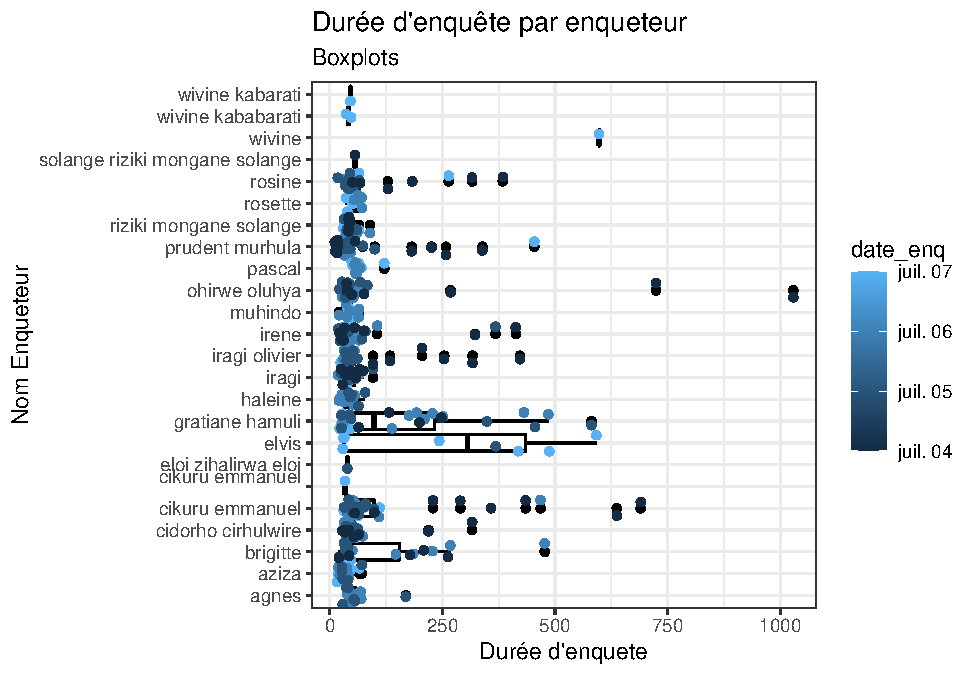
\includegraphics{IES_Endline_SPR_Book_files/figure-latex/unnamed-chunk-15-1.pdf}
De ce graphique, nous remarquons que le temps d'enquête diminue aussi la date avance

\hypertarget{methodologie}{%
\chapter{Methodologie}\label{methodologie}}

\hypertarget{muxe9thodologie-de-collecte-des-donnuxe9es}{%
\section{Méthodologie de Collecte des Données}\label{muxe9thodologie-de-collecte-des-donnuxe9es}}

\hypertarget{muxe9thodologie-danalyse}{%
\section{Méthodologie d'analyse}\label{muxe9thodologie-danalyse}}

\hypertarget{analyse-des-donnuxe9es}{%
\chapter{Analyse des données}\label{analyse-des-donnuxe9es}}

\hypertarget{description-des-donnuxe9es}{%
\section{Description des Données}\label{description-des-donnuxe9es}}

\hypertarget{construction-des-indicateurs-du-projet}{%
\section{Construction des indicateurs du Projet}\label{construction-des-indicateurs-du-projet}}

\hypertarget{construction-des-indicateurs-de-cohuxe9sion-sociale}{%
\section{Construction des indicateurs de Cohésion Sociale}\label{construction-des-indicateurs-de-cohuxe9sion-sociale}}

\hypertarget{conclusion}{%
\chapter{Conclusion}\label{conclusion}}

  \bibliography{book.bib,packages.bib}

\end{document}
